% Styling and set-up
\documentclass{article}


\usepackage{NotesStyle}
\graphicspath{./figs/}

% Cover info

\title{Phys 514 \\
	\large General Relativity}

\author{April Sada Solomon}
\date{Winter 2021}


% Document
\begin{document}

	\clearpage
	% Displays title info
	\maketitle
	
	\vspace{2cm}
	
	% Course description, displayed on cover page
	\renewcommand{\abstractname}{Course Description}
	\begin{abstract}
		 Notes taken directly from the lectures given by Dr. Maloney (not proof read by him). Special Relativity, Manifolds, Spacetime Curvature, Gravitation, Schwarzchild Solution, Black Holes, Perturbations, Radiation, Introduction to Cosmology, Introduction to QFT in Spacetime. 
	\end{abstract}
	
	\newpage
	
	\tableofcontents
	
	\newpage
	
	% Start page count after the TOC
	\setcounter{page}{1}
	\cfoot{\thepage}
	
	% Notes body
	\section{Introduction}
	\subsection{A Brief Review of Special Relativity}
	
		\textbf{Disclaimer:} This chapter should \textbf{not} be used to define the formalities that will be dealt with later. Rather, this chapter is meant to serve as a bridge coming from Special Relativity to have the conceptual framework to work with General Relativity. If you already feel comfortable with Special Relativity, \hyperref[ch:2]{skip to chapter 2}. Otherwise, I suggest reading this chapter before you begin.
	
 		General Relativity is the modern theory of classical gravity. What do we mean by "classical"? Simply, it is a nomenclature to distinguish from Quantum Mechanics, so those effects are ignored. The basic idea from Newtonian Mechanics is that gravity is a force, and as we know, most forces are described by fields.
 		
 		The simplest example of a field that describes a force is the Newtonian gravitational potential $\Phi (\vec{r})$:
 		\begin{equation}
 			\label{eq:NetwonGravitation}
 			\frac{d}{dt}\frac{\partial \Lgr}{\partial \dot{x}} = \frac{\partial \Lgr}{\partial x} \implies \vec{F} (\vec{v}) = - \frac{\partial}{\partial \vec{r}} \Phi (\vec{r}) 
 		\end{equation}
 		\noindent
 		If we are studying electromagnetism, we would study the electromagnetic fields $\vec{E}$ and $\vec{B}$. Let us list the Maxwell Equations, that we will review again later on:
 			\begin{align}
 				\label{eq:Maxwell}
 				\Del \cdot \vec{E} &= \frac{\rho}{\varepsilon_0} \\
 				\Del \cdot \vec{B} &= 0 \\
 				\Del \times \vec{E} &= -\frac{\partial \vec{B}}{\partial t} \\
 				\Del \times \vec{B} &= \mu_0 \left( \vec{J} + \varepsilon_0 \frac{\partial \vec{E}}{\partial t} \right)
 			\end{align}
 		A classical field theory like the theory of Newtonian gravity or the theory of Electromagnetism has two parts that describe it:
 		\begin{enumerate}
 			\item \textbf{Field equation}
 				\subitem A field equation is an equation of motion that describes exactly how a certain field is determined by some set of sources. In other words, it is usually a second order differential equation that has to be solved to determine the field from some collection of sources. 
 			\begin{exmp}
 				Newtonian gravity field equation
 				$$ \nabla^2 \Phi = 4\pi G \rho$$
 				where $\rho$ is the mass density. We solve this Laplace's equation to determine the field. If $\rho$ is a $\Del(\vec{r})$ function such that it describes a point mass, which implies that
 				$\Phi \propto \nicefrac{1}{\vec{r}}$.
 			\end{exmp}
 		\pagebreak
	 		\begin{exmp}
	 			Electromagnetic field equations. See the \hyperref[eq:Maxwell]{Maxwell's Equation's} above. In equation (1.2), we have that $\rho$ represents the charge density to determine the field in terms of the forces from some collection of charge sources.
	 		\end{exmp}
 			\item \textbf{Force law}
 			\subitem The force law is an equation that determines how an object moves in the presence of a field. So we start by describing a collection of sources and how they describe some force field, and then we use the force law to determine how bodies in motion are affected by the force field using the force law.
 			\begin{exmp}
 				Newtonian force law
 				$$ \vec{F}(t, \vec{x}, \dot{\vec{x}}) = \frac{m}{2}\frac{d}{dt} \frac{\partial}{\partial \vec{v}}\vec{v}^2 = m \dot{\vec{v}} =- m \vec{\Del} \Phi(t,\vec{x}) $$
 				where $\dot{\vec{v}} = \nicefrac{d^2 \vec{x}}{dt^2} = \ddot{\vec{x}}$. This force law describes how some gravitational potential affects the motion of bodies in the presence of the field described by the potential.
 			\end{exmp}
 			\begin{exmp}
 				Lorentzian force law
 				$$ \vec{F} \left(t, \vec{x}, \dot{\vec{x}}\right)=q (\vec{E} + \vec{v} \times \vec{B} )$$
 				where $\vec{v} = \nicefrac{d\vec{x}}{dt} = \dot{\vec{x}}$.
 			\end{exmp}
 			The important thing here is that fields are just functions of points in spacetime. For example, the gravitational potential $\Phi (t, \vec{x})$ yields a number that depends on where you are in space time, and the electric field $\vec{E} (t, \vec{x})$ is also a vector that depends on where you are in space and time. We should think of force laws as equations that describe how the motion of objects deviate from being "straight lines". 
 		\end{enumerate}
 		To emphasize, let us assume that an object in inertial motion on the $+\hat{x}$ axis, neglecting field interactions with the object. Evidently so, it's acceleration is zero, yielding the differential equation $\ddot{x} = 0$. The solution to this second order differential equation yields motion in a straight line. So the force law considering a field with an object experiencing this motion will be able to distort the object's motion such that it is not a straight line anymore. For instance, a gravitational field will bend the straight line into a curve as it generates acceleration in the $-\hat{y}$ axis, leading to parabolic motion on the $\hat{x}\hat{y}-$plane.
 		
 		\begin{defn}
 			\textbf{General Relativity} is a complete reinterpretation of gravitation such that it is not a field using a potential $\Phi (t, \vec{x})$, but instead it is a feature of spacetime itself. In particular, we replace the gravitational potential with a \textit{metric tensor} that describes this feature, particularly, the geometrical curvature of spacetime.
 		\end{defn} 
 		We will be learning pseudo-Riemann topological spaces by employing Einstein's field equation, which determines how spacetime curvature is determined in the presence of matter or energy. In Newtonian gravitation, the source term was a mass (or energy density in Special Relativity where $E = mc^2$). Recall however that mass has no independent meaning in terms of relativity as energy and momentum both depend on the reference frame where they are measured. The "source" of the curvature in general relativity is a term in the Einstein field equations that describes a generalized mass-energy distribution in spacetime of the sources present.
 		
 		The force law is also replaced by the geodesic equation, which tells us how objects move through some curved spacetime. Particularly, the geometric interpretation of the geodesic is quite simple; it is the statement that \textit{object will move on \textbf{geodesics}, which are the extremal paths on some manifold.} In a flat surface, this is a straight line, but in curved topologies, this trajectory will not be a straight line, like two points on the surface of a sphere.
 		
 		\begin{figure}[h]
 			\begin{subfigure}{0.46\textwidth}
 				\center
 				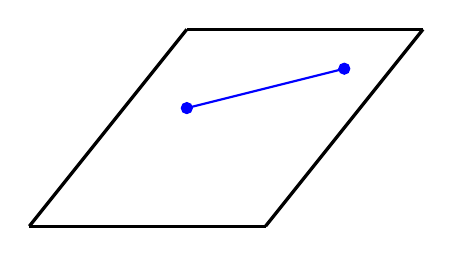
\begin{tikzpicture}
 					\draw [very thick] (-1,-2) -- (1,0.5);
 					\draw [very thick] (2,-2) -- (4,0.5);
 					\draw [very thick] (-1,-2) -- (2,-2);
 					\draw [very thick] (1,0.5) -- (4,0.5);
 					
 					\draw [thick, blue] (1, -0.5) -- (3, 0);
 					
 					\filldraw [blue] (1, -0.5) circle (2pt)
 					(3,0) circle (2pt);
 				\end{tikzpicture}
 			\vspace{0.5cm}
 			\caption{Geodesic over a flat surface}
 			\end{subfigure}
 			\begin{subfigure}{0.46\textwidth}
 				\center
 				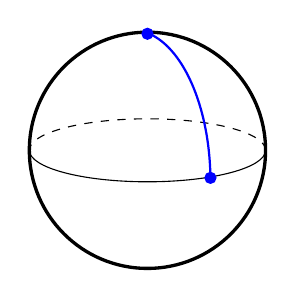
\begin{tikzpicture}
 					\draw [very thick] (0,0) circle (1.5cm);
 					\draw [dashed] (1.5,0) arc (0:180:1.5 and 0.4);
 					\draw (1.5,0) arc (0:180:1.5 and -0.4);
 					
 					\draw [thick, blue] (0.8, -0.35) arc (1.5:80:1 and 1.93);
 					
 					\filldraw [blue] (0.8,-0.35) circle (2pt)
 					(0,1.48) circle (2pt);
 				\end{tikzpicture}
 				\caption{Geodesic over a spherical surface}
 			\end{subfigure}
 			\caption{Examples of geodesic on different surfaces.}
 		\end{figure}
 		So in other words, it is the curve that finds the extrema of the distance between two points over some space. The force law is therefore just the statement that bodies will move in geodesics over some geometry, even when said geometry is curved. So when we think of gravity as the curvature of spacetime, then geodesics will describe motion over spacetime as it is curved.
 		
 		The discussion of special relativity will serve to introduce spacetime properly. We will develop it further later on, but for now we will proceed with a heuristic manner. 
 		
 		\begin{defn}
 			\textbf{Spacetime} is a smoothly connected manifold where the points defined are called \textbf{events}.
 		\end{defn}
 		The events in spacetime can be smoothly parametrized using coordinates, such as the most common system of coordinates used, the Cartesian coordinates.
 		\begin{exmp}
 			Cartesian coordinates
 			$$ (t, \vec{x}) = (-c\hat{t}, \hat{x}, \hat{y}, \hat{z})$$
 			In relativistic mechanics, we usually consider all directions of motion in a single vector $\vec{x} = (\hat{x}, \hat{y}, \hat{z})$ while time is multiplied by the negative speed of light $t = (-c\hat{t})$. We will explain this later on.
 		\end{exmp}
 		Thus, spacetime is a smooth manifold with events as points parametrized by some coordinates, and in relativity, we know that physics should be independent of its coordinate system. This is known as the \textbf{principle of general covariance}.
 		
 		\pagebreak
 		To begin, let us assume we are working with Newtonian mechanics where we have two points in spacetime labelled $(t_1, \vec{x}_1) = (t_1, x_1, y_1, z_1)$ and $(t_2, \vec{x}_2) = (t_2, x_2, y_2, z_2)$ respectively, both of which describe a single event in spacetime given as $$(\Delta t, \Delta \vec{x})$$ 
 		In this event, $\Delta t$ denotes the \textbf{temporal separation} while $\Delta \vec{x}$ denotes the \textbf{spatial separation}. Explicitly:
 		\begin{align*}
 			\Delta t &=	t_2 - t_1\\
 			\Delta \vec{x} &= \sqrt{(\vec{x}_2 - \vec{x}_1)\cdot (\vec{x}_2 - \vec{x}_1)}\\ 
 			&= \sqrt{(x_2 - x_1)^2 + (y_2 - y_1)^2 + (z_2 - z_1)^2} & (\text{in Cartesian coordinates})
 		\end{align*}
 		This makes sense as Newtonian mechanics can always be written in terms of both $\Delta t$ and $\Delta \vec{x}$, so the numerical value of $t_1$ will depend on the origin in the frame of reference we are working on. In other words, if we choose our reference frame to be Montreal at 6:00pm and remain at rest until 6:01pm, then we can denote that $\Delta t = 60$ s. So if we now jog in Montreal at constant velocity of $1$ m/s in this reference frame, the velocity will depend on the time separation $\Delta t$ and not on the absolute values of $t_1$ and $t_2$. So, if we suddenly change the time frame to be 4:20pm to 4:21pm, the velocity should not vary due to the absolute value of the new points in time, as the time separation $\Delta t$ would be the equal to the case at 6:00pm. The same would go for the choice of spatial coordinates, so if we move from Montreal to Toronto and the speed remains constant, the space separation $\Delta \vec{x}$ should also not vary. To summarize, the laws of physics would remain invariant even if we change the choice of reference frame where the choice of time is independent of the choice of space, and so they are independent of the entire coordinate system chosen. Albeit elementary to classical mechanics, it is vital to understand this properly to proceed with the philosophy of relativity.
 		
 		In special relativity, there is no separate notion between space and time, so we denote both as spacetime. This means that the both the separation of time and the separation of space are dependent on each other, which leads to effects like time dilation. Time dilation implies that \textit{the temporal difference $\Delta t$ of two event in spacetime will depend on the relative position in spacetime where an observer is viewing the event from}. Similarly, the distance or length of an object will depend on where the observer is in spacetime. In other words, we cannot think of $\Delta t$ and $\Delta \vec{x}$ as independent separations in spacetime, as one is directly related to the other depending on the frame of reference. So, observing the same event in a different reference frame will change the values of $\Delta t$ and $\Delta \vec{x}$. 
 		
 		However, we can denote an invariant notion to both the spatial and temporal separations called the \textbf{interval} between two events as
 		$$ \Delta s^2 = -c^2 \Delta t^2 + \Delta \vec{x}^2 \quad \quad (\text{in Cartesian coordinates})$$
 		Usually, we simplify by allowing $c=1$ in units in terms of the speed of light [$3\times 10^8$ m/s] such that
 		\begin{equation}
 			\label{eq:Interval}
 			\Delta s^2 = - \Delta t^2 + \Delta \vec{x}^2
 		\end{equation}
 		So when we measure distance with respect to the speed of light, we do so in terms of light-time, such as light-seconds and light-years. It is usually helpful to draw pictures in a spacetime diagram.
 		\begin{figure}[h]
 			\center
 			\begin{tikzpicture}[scale=1.6]
 				% Grid
 				\filldraw [green, opacity=0.25] (-3, 1) -- (-3, 3) -- (3,3) -- (3,2) -- (-0.5, -1.5);
 				\filldraw [green, opacity=0.25] (-1, -2) -- (-0.5, -1.5) -- (0,-2);
 				\filldraw [red, opacity=0.1] (-3,1) -- (-0.5, -1.5) -- (-1, -2) -- (-3, -2);
 				\filldraw [red, opacity=0.1] (3,2) -- (-0.5, -1.5) -- (0, -2) -- (3, -2);
 				\draw [step=0.5cm, grey, opacity=0.25] (-3,-2) grid (3,3);
 				% Axes
 				\draw [->, thick, >=stealth] (-0.5, -2) -- (-0.5, 2.5)
 				node [above] {$t$};
 				\draw [->, thick, >=stealth] (-3, -1.5) -- (2.5, -1.5)
 				node [right] {$x$};
 				\draw [->, thick,blue, >=stealth] (-0.62, -2) -- (0.5, 2.5)
 				node [above] {$t'$};
 				\draw [->, thick, blue, >=stealth] (-1.95, -2) -- (2.5, -0.5)
 				node [right] {$x'$};
 				% Light cone
 				\draw [green] (1.5, 2.85) node [] {Time-like, $s^2 < 0$} (1.5, 2.65) node [] {Future} (-0.33, -1.88) node [] {\smaller Past} ;
 				\draw [red] (2.5, 0) node [] {Space-like} (2.5,-0.23) node [] {$s^2 > 0$};
 				\draw [black] (2 , 1.3) node [] {\small$x = t$}
 				(-1.5,0)node [] {\small$x = -t$}
 				;
 				\draw [blue] (2.5 , 1) node [] {\small$x' = t'$}
 				(-2,-0.5)node [] {\small$x' = -t$}
 				;
 				\draw [very thick, olive] (-1, -2) -- (3, 2)
 				;
 				\draw [very thick, olive] (-3, 1) -- (0, -2);
 				% Event is the same
 				\draw [dashed] (-0.5, 1.5) -- (1.5, 1.5);
 				\draw [dashed] (1.5, -1.5) -- (1.5, 1.5);
 				\draw [dotted, thick, blue] (0.21, 1.2) -- (1.5, 1.5);
 				\draw [dotted, thick, blue] (0.7, -1.08) -- (1.5, 1.5);
 				\filldraw [black] (1.5, 1.5) circle (1.5pt) node [above=2mm] {\small Event}; 
 				
 			\end{tikzpicture}
 		\caption{A spacetime diagram of an time-like event with the light cone in two different reference frames, a static frame $K= (t,x)$ and another moving away from the static frame at a fraction of the speed of light, $K' = (t', x')$. Notice how even if the spatial ($\Delta x \neq \Delta x'$) and temporal ($\Delta t \neq \Delta t'$) separations vary from one reference frame to the other, the interval in spacetime remains invariant $\Delta s^2 = \Delta(s')^2$. We usually denote $(t_1, x_1) = (t_1', x_1') = (0,0)$ for convenience in either reference frame.}
 		\end{figure}
 	
 		Notice in the spacetime diagram that when $\Delta s^2 = 0$, we have that $\Delta x = \pm \Delta t$, defining a \textbf{light cone}. Events defined on the light cone are denoted \textbf{light-separated events} or \textbf{null-separated events}. As otherwise noted, events where $\Delta s^2 < 0 $ are inside the light cone and denoted as \textbf{time-like} or \textbf{time-separated}, while events where $\Delta s^2 > 0$ lie outside the light cone and are denoted as \textbf{space-like} or \textbf{space-separated}. Notice that for time-like events, it is clear that when $t_2 > 0$, the event will propagate to the future, while if $t_2 < 0$ it propagates to the past. Also note that space-like events are deemed as impossible, as there is no geodesic inside a light cone that can connect the origin to the event. In other words, an object would have to travel faster than light to arrive at this location in spacetime, which is indeed impossible in special relativity.
 		
 		We would get hyperbolic equilibrium to a 2D spacetime system with respect to the interval $\Delta s^2$. This means a time-like event will always be either time-like or get close to null-like, while a space-like event will also either remain space-like or get close to null-like. 
 	\pagebreak
 		\begin{claim}
 			We can reduce Special Relativity to the statement that for 2 time-like separated events, the proper time $\Delta \tau$ measured by an observer moving at constant velocity between the two events is given by:
 			$$ \left( \Delta \tau \right)^2  = - \left( \Delta s \right)^2$$
 		\end{claim}
 		
 		\begin{exmp}
 			\textbf{Time dilation}
 			\begin{figure}[h]
 				\begin{minipage}{0.4\textwidth}
 					\center
 					\begin{tikzpicture}[scale=1]
 						%\draw (2,2) node []{$\M$} ;
 						\draw [step=0.5cm, grey, opacity=0.25] (-2.5,-2.5) grid (2.5,2.5);
 						\draw [->, very thick,  blue, >=stealth] (-1,-2) -- (-1,1.95);
 						\draw [->, very thick, green, >=stealth] (-1,-2) -- (0.5,-0.05);
 						\draw [->, very thick, green, >=stealth] (0.5,0) -- (-0.95,1.95);
 						\draw [->] (-2, -2.5) -- (-2, 2) node (taxis) [above] {$t$};
 						\draw [->] (-2.5, -2) -- (2, -2) node (xaxis) [right] {$x$};
 						\filldraw (-1, -2) circle (2pt) node [right =2mm, below] {$A$}
 						(-1, 2 ) circle (2pt) node [right =2mm, above] {$C$}
 						(-1, 0) circle (2pt) node [right =2mm, below] {$B$}
 						(0.5, 0) circle (2pt) node [right =2mm, below] {$B'$};
 						\draw [<->, blue] (-1.5, -2) -- (-1.5, 2) node [left=2mm, below=1.9cm] {$\Delta t$};
 						\draw [<->, green, >=stealth] (-0.95, 0) -- (0.45, 0) node [left=0.8cm, above=-0.2mm] {$\Delta x$};
 					\end{tikzpicture}
 					\caption{Spacetime diagram for the twin's paradox. Notice that the inclination of the trajectory of the second twin is greater than $\nicefrac\pi4$ with respect to the $x$-axis, implying that the speed $v<c$.}
 				\end{minipage}
 				\hfill
 				\begin{minipage}{0.56\textwidth}
 					\begin{spacing}{1.5}
 						Here, we see the famous \textit{twin's paradox}. We have two observers relative to a frame of reference, usually considered twins, that will go from a point $A(t,x) = (0, 0)$ to a point $C(t,x)=(\Delta t, 0)$ in spacetime. The first twin will remain static in space while the second will go to point $B' (t,x) = \left(\frac{\Delta t}{2}, \Delta x\right)$ before reaching point $C$, where $\Delta x = \frac12 v \Delta t$ for constant propagation velocity $v$. The proper time for the trajectory of the first twin from $A$ to $B$ is clearly $\tau_{B,A} = \frac{\Delta t}{2}$, but for the second twin, the proper time from $A$ to $B'$ is given by
 					\end{spacing}
 				\end{minipage}
 			\end{figure} 
 			\vspace{-0.5cm}
 			$$ \tau_{B',A}^2 = \left(\frac{\Delta t}{2}\right)^2 - (\Delta x)^2 $$
 			\begin{equation}
 				\label{eq:RelativeProperTime}
 				\therefore \boxed{\tau_{B',A} = \frac{\Delta t}{2} \sqrt{1 - v^2} }
 			\end{equation}
 			
 			By symmetry, it follows that $\tau_{C,B} = \tau_{B,A}$ and $\tau_{B', A} = \tau_{C, B'}$. Considering the entire sequence of movement for both twins, we have
 			\begin{align*}
 				\tau_{C,B,A} &= \Delta t \\
 				\tau_{C,B',A} &= \sqrt{1 - v^2} \Delta t
 			\end{align*}
 			Clearly, $\tau_{C,B,A} > \tau_{C,B',A}$, and so the second twin is younger than the first twin by the time they both reach the point $C$. This implies that the proper time $\tau$ along some world line is related to the interval $\Delta s^2$ traversed through spacetime. Therefore, we can assess the ratio of relative time difference between the twins as 
 			
 			$$ \frac{2 \tau_{C,B',A}}{\tau_{C,B,A}} = \sqrt{1-v^2} $$
 		\end{exmp}
 	\pagebreak
 		\begin{exmp}
 			\textbf{Length contraction} 
 			\begin{figure}[h]
 				\begin{minipage}{0.4\textwidth}
 					\center
 					\begin{tikzpicture}[scale=1]
 						%\draw (2,2) node []{$\M$} ;
 						\draw [step=0.5cm, grey, opacity=0.25] (-2.5,-2.5) grid (2.5,2.5);
 						
 						\draw [->] (-2, -2.5) -- (-2, 2) node (taxis) [above] {$t$};
 						\draw [->] (-2.5, -2) -- (2, -2) node (xaxis) [right] {$x$};
 						
 						\draw [->, very thick, blue,>=stealth] (-2,-2) -- (-1, 2)
 						 node [left=9mm, below=10mm] {$x=vt$};
 						\draw [->, very thick, green, >=stealth] (-2,-2) -- (0.5, 0.5)
 						 node [left=13mm, below=5mm] {$x=t$};
 						\draw [->, very thick, green, >=stealth] (0.5, 0.5) -- (-1,2)
 						 node [right=12mm, below=0mm] {$x=2L-t$};
 						
 						\draw [very thick] (0.5, -2) -- (0.5, 2.5);
 						\draw [very thick, red] (-2, -2) -- (0.5, -2);
 						\filldraw [red] (-2,-2) circle (1pt) node [below=3mm, right] {$(0,0)$}
 						(0.5, -2) circle (1pt) node [below] {$(0,L)$};
 						\filldraw [green] (0.5, 0.5) circle (1.5pt) node [right] {$(L,L)$};
 						\filldraw [black] (-1, 2) circle (1.5pt) node [above] {$(t_2, x_2)$};
 					\end{tikzpicture}
 					\caption{The spacetime diagram for length contraction. }
 				\end{minipage}
 				\hfill
 				\begin{minipage}{0.56\textwidth}
 					\begin{spacing}{1.5}
 						Consider an observer moving at constant velocity $v$ from the origin of a reference frame  with respect to a static ruler with a light bulb at the point $(0,0)$. We would like for the observer to measure the ruler using light-travel time, which is achieved by flashing the light bulb and measuring the time it takes to reach a point $(L,L)$, and return to the observer at the intersection point $(t_2, x_2)$. Noting how we have two solutions for $x$, namely $x = 2L-t$ and $x=vt$, we can equate them to find $(t_2, x_2)$ such that
 					\end{spacing}
 				\end{minipage}
 			\end{figure} 
 			\vspace{-1cm}
 			\begin{align*}
 				t_2 &= \frac{2L}{(1+v)}\\
 				x_2 &= v \left( \frac{2L}{(1+v)} \right)
 			\end{align*}
 			And so, the proper time $\Delta \tau^2$ measured by the observer at the point when the light bulb's ray is reflected back is given by $\Delta \tau^2 = \Delta t^2 - \Delta x^2$ such that
 			$$ \Delta \tau^2 = \left(\frac{2L}{(1+v)}\right)^2(1 - v^2)$$
 			Knowing that an observer at rest with the ruler $\Delta t^2$ for the light to reflect back on itself is $\Delta t = \frac{2L}{(1+v)}$, we get the ratio
 			$$ \frac{\Delta \tau^2}{\Delta t^2} = (1-v^2)$$
 			So the apparent length of the ruler would be shorter by a factor of $v^2$. Note that in the case where $x = -vt$ for the observer's trajectory, the same ratio would arise.
 		\end{exmp}
	 	We are very habituated to writing the interval in the following way
	 	$$ \Delta s^2 = - \Delta t^2 + \Delta x_1^2 + \Delta x_2^2 + \Delta x_3^2$$
	 	We will consider the $x^\mu$ notation, where $\mu=0,1,2,3$, to denote these coordinates as a single coordinate. Moreover, we can denote $x^i$ where $i=1,2,3$ as the spatial coordinates. Therefore, we may define
	 	\begin{multicols}{4}
	 		\begin{itemize}
	 			\item $x^0 = t$
	 			\item $x^2 = x_2$
	 			\item $x^1 = x_1$
	 			\item $x^3 = x_3$
	 		\end{itemize}
	 	\end{multicols}
	 	We can thus summarize the coordinates of some interval to a summation
	 	$$ \Delta s^2 = \sum_{\mu=\nu} \eta_{\nu\mu}\Delta x^\mu \Delta x^\nu$$ 
	 	Where we define $\eta_{\mu\nu}$ to be a $4\times4$ diagonal matrix such that
	 	$$ \eta_{\mu\nu} = \begin{pmatrix}
	 		-1	&	0	&	0	&	0\\
	 		0	&	1	&	0	&	0\\
	 		0	&	0	&	1	&	0\\
	 		0	&	0	&	0	&	1
	 	\end{pmatrix}$$ 
	 	\begin{defn}
	 		The \textbf{metric} of flat spacetime in Cartesian coordinates is given by the $4 \times 4$ matrix $\eta_{\mu\nu}$.
	 	\end{defn}
	 	We may further simplify the interval by using \textit{Einstein summation notation}. This notation takes the summation symbol for granted, which adds all terms in the resulting $4\times4$ matrix whose indices follow the property $\mu=\nu$, to get
 		\begin{equation}
 			\label{eq:IntervalEinstein}
 			\Delta s^2 = \eta_{\mu\nu} \Delta x^\mu \Delta x^\nu
 		\end{equation}
 		As such, in tensor calculus language this implies that for every subscript in a tensor we must have a corresponding superscript to yield an interval as desired. In this case, $\eta_{\mu\nu}$ has two subscripts, each denoting an index for the matrix, and the one-forms $\Delta x^\mu$ and $\Delta x^\nu$ each have one superscript to indicate their contravariant components. Hence, we can summarize special relativity to the statement that all intervals in spacetime can be given by an equation in the form of (\ref{eq:IntervalEinstein}), such that spacetime is denoted as \textbf{Minkowski spacetime} $\R^{1,3}$ or simply $\M$. To summarize for now, general relativity implies that spacetime can be something other than Minkowski spacetime $\M$.
 		
 		Other examples of spaces are Euclidean spaces, both in 2D ($\R^2$) and in 3D ($\R^3$), where an invariant interval is simply denoted as the distance between two points. Using the notation we have established, the coordinates in 2D and 3D respectively would be:
 		\begin{align*}
 			(x^1, x^2) &= (x,y) \\
 			(x^1, x^2, x^3) &= (x,y,z)
 		\end{align*}
 		For either of these, the distance is obtained by use of Pythagoras's theorem $D = \sqrt{(x^1)^2 + (x^2)^2 + (x^3)^3}$, where in 2D we simply neglect the $x^3$ term. Recall than an invariant interval is similarly given by $\Delta s^2 = -(x^0)^2 + (x^1)^2 + (x^2)^2 + (x^3)^3$.
 		where the $x^0$ term is given a negative sign. Note that an opposite yet equally valid for the invariant interval is $\Delta s^2 = \Delta t^2 - \Delta x^2 $. This convention is better for events happening in the same spatial coordinate at different points in time, while the one we used is better for events that happen at the same time in different spatial coordinates.
 		\begin{exe}
 			Recalling that a Lorentzian transformation $\Lambda$ is a linear change of coordinates, determine the correct form of the $2 \times 2$ matrix $\Lambda$ that validates the following change of coordinates:
 			$$ \begin{bsmallmatrix}
 				x \\
 				t
 			\end{bsmallmatrix} \to \begin{bsmallmatrix}
 			x' \\
 			t'
 			\end{bsmallmatrix} = \Lambda \begin{bsmallmatrix}
 			x\\t
 		\end{bsmallmatrix}$$
 		\end{exe}
 		
 		To summarize, the proper time $\Delta \tau$ measured by an observer moving at some constant velocity $v$ between two points in spacetime is given by
 		$$ (\Delta \tau)^2 = - (\Delta s)^2 = \Delta t^2 - \Delta \vec{x}^2$$
 		Where we could write the invariant interval $\Delta s^2$ using Einstein summation notation as 
 		$$ \Delta s^2 = \eta_{\mu\nu} \Delta x^\mu \Delta x^\nu$$
 		For the coordinates $\Delta x^\mu = (\Delta t, \Delta \vec{x})$ where $\mu = 0,1,2,3$, and the metric $\eta_{\mu\nu}$. Recall that this notation neglects a summation symbol that will sum all elements in the $4\times4$ matrix $\eta_{\mu\nu} \Delta x^\mu \Delta x^\nu$ that follow the property $\mu = \nu$.
 		
 		Thus far, we have only considered an observer moving at constant velocity for the sake of conceptual simplicity. However, when consider gravitation we will encounter accelerating reference frames. That is, we will encounter motion in spacetime that is not given by a straight line, but rather by some curve, implying variable velocity. 
 		\begin{defn}
 			A general path through spacetime is denoted as a \textbf{worldline} and can be parametrized with 4 functions, one for each coordinate in the metric.
 		\end{defn}
 		\begin{figure}[h]
 			\begin{minipage}{0.4\textwidth}
 				\center
 				\begin{tikzpicture}[scale=1]
 					%\draw (2,2) node []{$\M$} ;
 					\draw [step=0.5cm, grey, opacity=0.25] (-2.5,-2.5) grid (2.5,2.5);
 					
 					\draw [->] (-2, -2.5) -- (-2, 2) node (taxis) [above] {$t$};
 					\draw [->] (-2.5, -2) -- (2, -2) node (xaxis) [right] {$x$};
 					\draw [thick, dashed, green] (-2,-2) -- (2.5, 2.5) node [below=20mm, left=5mm] {$\Delta s^2 = 0$};
 					 
 					\draw [thick, blue] plot [smooth] coordinates{(-2,-2) (-1, -0.75) (0, 0.5) (-0.5, 1) (-1, 1.5)};
 					\draw [line width=0.6mm, red] plot [smooth] coordinates{(-0.05, 0.4) (0, 0.5) (-0.05, 0.7) (-0.1, 0.7)} 
 					node [right] {ds};
 					
 					
 					\filldraw (-2, -2) circle (2pt) (-1,1.5) circle (2pt);
 				\end{tikzpicture}
 				\caption{A worldline in spacetime of a time-like observer accelerating, with a line element shown. Notice how at every point on the worldline, the observer's speed has the property $v<c$.}
 			\end{minipage}
 			\hfill
 			\begin{minipage}{0.56\textwidth}
 				\begin{spacing}{1.5}
 					The parametrization in Cartesian coordinates for a worldline using $\lambda$ as the variable which denotes points along the world line is as follows:
 					$$ x^\mu (\lambda) = \left(t(\lambda), x^1 (\lambda), x^2(\lambda), x^2 (\lambda)\right)$$
 					Along this worldline, we consider infinitesimally small displacements through space $d\vec{x}$ and through time $dt$ such that at each interval of displacement we approximate to constant velocity. The proper time $\Delta \tau$ measured by such an accelerating observer along a worldline is hence given by $\sqrt{-(\Delta s)^2}$, where
 				\end{spacing}
 			\end{minipage}
 		\end{figure}
 		\vspace{-1cm}
 		$$ \Delta s = \int \sqrt{ - \left(\frac{d x^0}{d \lambda}\right)^2 + \left(\frac{d x^1}{d \lambda}\right)^2 + \left(\frac{d x^2}{d \lambda}\right)^2 + \left(\frac{d x^3}{d \lambda}\right)^2} d \lambda$$ 
 		Which is simply the arc length of a curve, as expected. We could also write this using Einstein summation convention to make it cleaner:
 		$$ \Delta s = \int \sqrt{\eta_{\mu \nu} \frac{dx^\mu}{d\lambda} \frac{dx^\nu}{d\lambda}}d\lambda$$
 		For convenience, we will denote either of the above as
 		$$ \Delta s = \int ds$$Where we define $ds$ as the \textbf{line element} of a worldline, given by
 		\begin{equation}
 			\label{eq:LineElement}
 			\boxed{ds^2 = \eta_{\mu\nu} dx^\mu dx^\nu}
 		\end{equation}
 		We think of $ds$ as an infinitesimal variation on the interval $\Delta s$, and so $dx^\mu$ and $dx^\nu$ are infinitesimal displacements on the coordinates $x^\mu$.
 		
 		We again redefine Special Relativity to the statement that the line element is given by equation (\ref{eq:LineElement}), where we defined $\eta_{\mu\nu}$ as a metric given by a $4\times4$ diagonal matrix with constant components. In General Relativity we have the statement that all of the effects of gravity are packaged in terms of a replacement 
 		$$ \eta_{\mu\nu} \to g_{\mu \nu} (x)$$
 		Which is a $4\times4$ matrix, formally called a tensor, whose components can change according to the value of the coordinates given, rather than remaining constant as in Special Relativity. we denote $g_{\mu \nu}(x)$ as the \textbf{metric of curved spacetime}. This metric is parametrized by 16 functions of the coordinates of spacetime; one parametrization per component in the matrix. So the line element in General Relativity changes to
 		$$ ds^2 = g_{\mu\nu} dx^\mu dx^\nu$$
 		\begin{exmp}
 			\textbf{Light-rays in General Relativity}\\
 			
 			When we consider General Relativity, light propagation still takes the form of a \textit{null-like} worldline. However, the definition of null-like worldline, considering $ds^2 = 0$.
 		\end{exmp}
 		\begin{exmp}
 			\textbf{Massive objects in General Relativity}
 			
 			Massive objects in general relativity travel along \textit{time-like} worldlines such that $ds^2 < 0$, implying that their speed along a world line has the property $v<c$ at every point. This implies that the proper time $\Delta \tau^2$ measured by an observer in GR travelling along some worldline $x^\mu (\lambda)$ is given by
 			$$ \Delta \tau^2 = - \Delta s^2$$
 			Where we have
 			$$ \Delta s = \int ds = \int \sqrt{g_{\mu\nu} \frac{dx^\mu}{d\lambda} \frac{dx^\nu}{d\lambda}}d\lambda$$
 		
 		\end{exmp}
 	\pagebreak
 		We can now see why we say that Special Relativity is just the case of General Relativity where we will have a constant metric. And so, every case in Special Relativity can be solved with this form of a line element. Recall that all of this merely serves as a review of the study of Special Relativity such that we may introduce General Relativity, so we still need to formalize what has been stated.
 		
 		\subsection{Equivalence Principle}
 		
 		We will now introduce the \textbf{equivalence principle}. Recall the motion of objects in the presence of a gravitational potential in Newtonian gravitation:
 		$$ \vec{F}(\vec{v}) = m_i \dot{\vec{v}} = - m_g \vec{\Del}\Phi$$
 		We usually assumed that the inertial mass $m_i$, the mass due to the forces interacting with an object, and the gravitational mass $m_g$, the mass due to the gravitational potential interacting with the object were equivalent, and approximately speaking in human scales, they are. However, it is not true that we can say this generally. For every object and type of matter we know, both $m_i$ and $m_g$ are equal, but we do not know if all unknown objects will follow this rule. Given current evidence, we can cancel both masses out to assume that, for all objects known,
 		$$ \dot{\vec{v}} = \vec{a} = - \vec\Del \Phi$$
 		So the acceleration of an object will be independent of its mass, and as stated before, this is considered as an observational fact. In a gravitational potential, there are trajectories defined by the solutions to the equations of motion due to the potential on some object, denoted as \textbf{free-falling} or \textbf{inertial} trajectories, where no forces are interacting with an object. In a free-falling object, the object only experiences gravitational potential.
 		
 		Now, consider an infinitesimally small region where $\vec{\Del}\Phi \approx -\vec{a}_0$, where $\vec{a}_0$ is some constant to within some approximation made by measurements. 
 		
 		\begin{defn}
 			\label{defn:WeakEquivalence}
 			The \textbf{weak equivalence principle} states that in this small region, the effects of gravity are indistinguishable from the effects of a constantly accelerating reference frame.
 		\end{defn}
 	
 		\begin{exmp}
 			\textbf{Acceleration Experiment} \\
 			Let us imagine that we are in a laboratory on Earth as our frame of reference, which is very small. We can thus approximate the gravity with a downwards pull in this laboratory to be constant to some significant figure. The downwards gravitational force we experience within the lab is given by
 			$$ \vec{F}_g = -m g = - G \frac{mM_E}{R_E^2}$$
 			Where $G \approx 6.7 \times 10^{-11}\,\,\, \nicefrac{\text{N$\cdot$m}^2}{\text{kg}^2}$ is the gravitational constant, $M_E \approx 6.0\times 10^{24}$ kg is the mass of the Earth and $R_E \approx 6.4 \times 10^7$ m is the radius of the Earth as measured in this lab, so we assume that $g = 9.8 \,\,\, \nicefrac{\text{m}}{\text{s}^2}$.
 			\pagebreak
 			
 			\noindent
 			We can write this in a more mathematical manner as
 			$$ \ddot{x} = -g = -9.8 \,\,\, \nicefrac{\text{m}}{\text{s}^2}$$
 			Now, assume that we take this laboratory into a spaceship such that the laboratory is experiencing no gravitational force from Earth. However, the spaceship that contains the lab is experiencing upwards acceleration of $a_0 = g = 9.8 \,\,\, \nicefrac{\text{m}}{\text{s}^2}$, and thus so is the laboratory. This would imply that the normal acceleration experienced by us inside the lab would be $a_n = -g = -9.8 \,\,\, \nicefrac{\text{m}}{\text{s}^2}$. Clearly, this would mean that the effects of gravity would be indistinguishable from those of the accelerating spaceship if we were to perform mechanical experiments. In fact, pilots use this technique to accelerate upwards and downwards to simulate zero gravity. You can watch Stephen Hawking in such a plane ride \href{https://www.youtube.com/watch?v=OhIpdSZQZlI}{here}\footnote{Please forgive the potato quality as it is a 14 year old video as of the time of this writing.}. In more mathematical sense, we notice that the spaceship frame of reference is not inertial. The coordinates we define are thus accelerating when defined. To find the new $x'$, we first consider constant acceleration:
 			$$ \dot{x} \frac{dx}{dt} = -g$$
 			$$ \therefore \dot{x} \int_0^1dx = -g\int_0^tdt$$
 			We are considering the initial position in spacetime $x$ and wish to find a new position $x'$ relative to the acceleration. We integrate to find their difference with respect to time such that
 			$$\int_x^{x'} dx = -g \int_0^t t dt $$
 			$$ \therefore x' = x - \frac12gt^2$$ 
 			Where we have that $(t,x)$ are the usual spacetime coordinates outside the the laboratory and $(t, x')$ are the coordinates inside the lab as it is accelerating upwards. Hence, it becomes clear that
 			$$ \ddot{x} = \ddot{x}' = -g$$
 			\begin{defn}
 				The forces generated due to acceleration are denoted as \textbf{fictitious forces}.
 			\end{defn}
 			The main idea behind the equivalence principle is that inside a small frame of reference, the forces of Earth's gravity are roughly equivalent to the fictitious forces of the same frame accelerating in spacetime at $9.8 \,\,\, \nicefrac{\text{m}}{\text{s}^2}$. We can extend this to other gravitational sources aside from the Earth. As a result, we have that the metric of Minkowski space $\eta_{\mu\nu}$ will no longer be constant in terms of the accelerating frame of reference, and moreover, it implies that gravity itself is a result of the variance of the metric.
 		\pagebreak
 			
 			Once we assume that gravitational potential will vary over a larger region than we defined on the previous reference frames, for example in an entire planet or a star, we cannot think of gravity as a fictitious force. So imagine that the mighty nation of Canada decided to build a colossal completely flat spaceship of around 200 km in length over the continental United States, such that the corners of the ship are above the surface by around 800 m, while the centre rests in contact with the surface.
 			Thus, if we measure the gravitational force of the Earth along various points along the spaceship, we will find that the gravitational force is not constant if we are being precise. If we then reach space and accelerate the entire ship upwards relative to the Earth's frame of reference at exactly $9.8 \,\,\, \nicefrac{\text{m}}{\text{s}^2}$, we cannot say that the accelerating frame of the ship has an equivalent fictitious force to that of the gravity of Earth, as there are several points where gravity will not be equal. 
 			
 			\begin{defn}
 				\label{defn:StrongEquivalence}
 				The \textbf{strong equivalence principle} or \textbf{Einstein equivalence principle} states that in a small enough frame of reference, the laws of physics reduce to those of special relativity. Moreover, spacetime locally looks like Minkowski space.
 			\end{defn}
 		
 			Once we review differential geometry and tensors, we will be able to redefine this principle yet again to a much more mathematical version:
 			
 				\textit{For any point given by some coordinates $x_0^\mu$ in space time, there exists a coordinate system such that the line element takes that of special relativity near that specific point $x_0^\mu$. }
 				$$ ds^2 = \eta_{\mu\nu} dx^\mu dx^\nu + \mathcal{O}(x-x_0^\mu) $$
 		\end{exmp} \noindent
 		Where $\mathcal{O} (x-x_0^\mu)$ denotes the error in regard to the extent at which gravity is not a fictitious force.
 		\begin{exe}
 			Determine the expression for a line element $ds^2$ in terms of the accelerating coordinates in Example 1.10, as given by
 			\begin{align*}
 				x' &= x - \frac12 gt^2 \\
 				t' &= t
 			\end{align*}
 		\end{exe}
 	\pagebreak
 	\section{Pseudo-Riemannian Geometry} \label{ch:2}
 	\subsection{Manifolds}
 		We recall the equivalence principle which states that spacetime locally looks like Minkowski space $\R^{3,1}$. In small frames of reference we can presume that gravity can be ignored and thus assume a pure Minkowski space with accelerating frames of reference. In larger frames of reference, gravity does not act as a fictitious force, but the knowledge that it indeed is equivalent to a fictitious force is important nonetheless. To understand this. take the coordinate system we usually employ on the Earth itself of latitude and longitude. When we consider a local area as seen by a human being, these coordinates can be presumed to be in a flat space. However, when considering the same coordinates over larger distances as when travelling in a Trans-Atlantic flight, the metric describing the coordinates curves with the Earth itself.
 		
 		\begin{thm}
 			Spacetime is a 4-dimensional pseudo-Riemann manifold.
 		\end{thm}
 	
 		Because we are physicists, we will not prove this statement and instead consider it to be true while justifying it along the way with various concepts. For a more thorough analysis a book on differential geometry is highly recommended, but is not necessary for the following content.
 		
 		\begin{defn}
 			A $D$-dimensional\textbf{ manifold} $M$ is a set of points that can be labelled by coordinate systems in a smooth way.
 		\end{defn}
 		
 		We will assume all manifolds in this context to be smooth henceforth. 
 		
 		\begin{defn}
 			A \textbf{coordinate system} is a set of $D$ functions $x^i$ which label different points along the manifold $M$ in some region $U \subset M$ in a unique way. More precisely,
 			$$ x^i : U \to \R^D \quad \text{for }i=1,\dots,D $$
 		\end{defn}
 		\begin{defn}
 			The region $U$ which the coordinates label uniquely is called \textbf{coordinate patch} of some manifold $M$. We say that the manifold $M$ is covered by the coordinates $x^i$.
 		\end{defn} 
 		\begin{defn}
 			\textbf{Global coordinate systems} are the coordinate systems which cover all of $M$ such that $U \equiv M$. 
 		\end{defn}
 		Generally, many coordinate systems cover some patch $U \subset M$ while not all of $M$ and remain useful in various cases.
 		\begin{exmp}
 			Assume that we have two coordinate systems $x^i$ and $x^j$ where $i,j = 1,\dots, D$ which correspond to different ways of labeling a patch $U \subset M$. We can then write the coordinate transformation between $x^i$ and $x^j$ in two ways:
 			$$ x^i (x^j) \quad \text{or} \quad x^j (x^i)$$
 			Where both of these are infinitely differentiable functions everywhere on the manifold $M$.
 		\end{exmp}
 		The first observation we make is the following: 
 		\begin{thm}
 			If some two coordinate systems $x^i$ and $x^j$ uniquely label some points in a patch $U \subset M$, then we know that the Jacobian matrix $J$ of this coordinate transformation is invertible, where
 			$$ J = \frac{\partial x^i}{\partial x^j}$$
 		\end{thm}
 		\begin{cor}
 			The determinant of an invertible matrix is nonzero. Therefore,
 			$$ \det (J) \neq 0$$
 		\end{cor}
 		\begin{cor}
 			If $\det(J)=0$ then one of the coordinate systems is implied to be \textbf{degenerate}, or \textbf{singular}, such that it no longer labels points in $U \subset M$ uniquely. 
 		\end{cor}
 		\begin{exmp}
 			\textbf{2D Manifold}\\
 			Consider the manifold $M=\R^2$. We define two different sets of coordinates given by
 			\begin{align*}
 				(x,y) &\quad \text{Cartesian coordinates} \\
 				(r, \theta) &\quad \text{Polar coordinates}
 			\end{align*}
 			We find that the Cartesian coordinates are global for the manifold $M$, as any point in the manifold can be described by a point in Cartesian coordinates. However, the Polar coordinates are not global as they label all points in the Manifold except the origin. Notice that at the Cartesian origin $x=y=0$ it follows in the change of coordinates that $\theta$ no longer parametrizes the manifold, and so the coordinate system degenerates into $r$ only. To see this, let us set up the coordinate systems such that
 			\begin{align*}
 				x^i &= (x^1, x^2) = (x,y) \\
 				x^j &= (x^{1'}, x^{2'}) = (r, \theta)
 			\end{align*}
 			We can therefore write $x^i(x^j)$ and $x^j (x^i)$as
 			\begin{align*}
 				x^1(x^j) &= x^{1'} \cos x^{2'} = r\cos\theta  & x^{1'}(x^i) &= \sqrt{(x^1)^2 + (x^2)^2} = \sqrt{x^2 + y^2}\\
 				x^2 (x^j) &= x^{1'} \sin x^{2'} = r\sin \theta & x^{2'} (x^i) &= \arctan \left( \frac{x^2}{x^1} \right) = \arctan \left( \frac{y}{x} \right)
 			\end{align*}
 			Now, we build the Jacobian $J = \frac{\partial x^i}{\partial x^j}$ and take its determinant:
 			\begin{align*}
 				\det(J) &= 	\begin{vmatrix}
 					\frac{\partial x^1}{\partial x^{1'}} & \frac{\partial x^1}{\partial x^{2'}} \\
 					\frac{\partial x^2}{\partial x^{1'}} & \frac{\partial x^2}{\partial x^{2'}}
 				\end{vmatrix} =
 				\begin{vmatrix}
 					\frac{\partial x}{\partial r} & \frac{\partial x}{\partial \theta} \\
 					\frac{\partial y}{\partial r} & \frac{\partial y}{\partial \theta}
 				\end{vmatrix} = \begin{vmatrix}
 					\cos \theta & -r \sin \theta \\
 					\sin \theta & r\cos\theta
 				\end{vmatrix}
 			\end{align*}
 		\pagebreak
 			$$ \therefore \det(J) = r^2 \left( \cos^2 \theta + \sin^2 \theta \right) = r^2$$
 			We see that the $\theta$ components get cancelled such that $r^2 = 0 \implies \det(J) = 0$, as if the determinant is zero we have that $\cos^2 \theta + \sin^2 \theta \neq 0$. This effectively shows that Polar coordinates are not global coordinates, as they degenerate at the origin. However, we still find a lot of use for this coordinate system.
 			\begin{exe}
 				Compute the Jacobian $J' = \frac{\partial x^j}{\partial x^i}$ and find its determinant. Discuss the difference between both Jacobians $J$ and $J'$.
 			\end{exe}
 		\end{exmp}
 		When describing spacetime, we use a special notation for the coordinates in general relativity. We write $x^\mu$ for $\mu = 0,1,2,3$ when considering a spacetime manifold rather than $x^i$ for $i=1,2,3$ when considering Euclidean manifolds.
 		\begin{exmp}
 			\textbf{cartesian coordinates of flat Minkowski spacetime}
 			$$ x^\mu = (t, \vec{x}) \in \R^{1,3}$$
 		\end{exmp}
 	
 	\subsection{Principle of General Covariance}
 		\begin{defn}
 			\label{defn:GeneralCovariance}
 			The \textbf{Principal of General Covariance} requires that we write the laws of physics in such a way that any physical prediction made by these laws is independent of the choice of coordinate system to write that law.
 		\end{defn}
 		
 		The statement above is incredibly important. In order to write any physical law, we need to describe a set of coordinates to denote points in spacetime. However, what we want is that the outcome of every experiment be independent of any choice of coordinates chosen. It might seem obviously intuitive, but it is rather important to understand the mathematics behind General Relativity, as Einstein's field equations arise from this very principle, and thus, so does the theory of Generalized Relativity.
 		
 		The effect of the principle of General Covariance is that we need to understand now how various objects can transform under these changes of coordinates, so the laws we write must faithfully obey this principle. 
 		
 		\begin{exmp}
 			\textbf{Line element of Minkowski space (revisited)}\\
 			Recall the line element of Minkowski space:
 			$$ ds^2 = \eta_{\mu\nu} dx^\mu dx^\nu$$
 			Now, consider the change of coordinates $x^\mu \to x^\alpha (x^\mu)$ such that we have
 			\begin{align*}
 				dx^\mu = \left(\frac{\partial x^\mu}{\partial x^\beta} \right) dx^{\beta}
 			\end{align*} 
 			Recall that as we are using Einstein notation, the differential of the first coordinate system is indeed a set of 4 equations where $\mu=0,1,2,3$ such that
 			\begin{equation}
 				\label{eq:JacobianChange}
 				\boxed{dx^\mu = \sum_{\beta = 0 }^3 \left(\frac{\partial x^\mu}{\partial x^\beta} \right) dx^\beta =  \left(\frac{\partial x^\mu}{\partial x^\beta} \right) dx^{\beta}}
 			\end{equation}
 			Which in total implies 16 terms, 4 per equation.
 			Recall the Cartesian and Polar coordinates in a 2D manifold given by
 			\begin{align*}
 				x &= r \cos \theta  \\
 				y &= r \sin \theta
 			\end{align*}
 			The differentials of the Cartesian coordinates as given by equation (\ref{eq:JacobianChange}) in this case are
 			\begin{align*}
 				dx &= \left(\frac{\partial r\cos \theta}{\partial r} \right)  + \left(\frac{\partial r\cos \theta}{\partial \theta} \right)= \cos \theta dr - r\sin\theta d\theta \\
 				dy &= \left(\frac{\partial r\sin \theta}{\partial r} \right) + \left(\frac{\partial r\sin \theta}{\partial \theta} \right) = \sin \theta dr + r\cos\theta d \theta
 			\end{align*}
 			Without loss of generality, the line element of flat Minkowski space in terms of some coordinates $x^\alpha$ to change from some given coordinates $x^\mu$ would be given as
 			\begin{align*}
 				ds^2 &= \eta_{\mu\nu} dx^\mu dx^\nu \\
 				& = \left( \frac{\partial x^\mu}{\partial x^\alpha} dx^\alpha \right) \left( \frac{\partial x^\nu}{\partial x^\beta} dx^\beta \right) \eta_{\mu\nu}
 			\end{align*}
 			We now rewrite the coordinate change with the metric $\eta_{\mu\nu}$ itself to get
 			\begin{equation}
 				\label{eq:MetricVariance}
 				\boxed{g_{\alpha \beta} = \eta_{\mu\nu}\frac{\partial x^\mu}{\partial x^\alpha}\frac{\partial x^\nu}{\partial x^\beta} }
 			\end{equation}
 			Which yields the cleaner version of the line element as denoted by
 			\begin{equation}
 				\label{eq:FlatMinkowskiLineElement}
 				\boxed{ds^2 = g_{\alpha \beta} dx^\alpha dx^\beta =\eta_{\mu\nu} dx^\mu dx^\nu }
 			\end{equation}
 			we are hence given the metric transformation $\eta_{\mu\nu} \to g_{\alpha \beta}$.
 			Again, recall the case of a 2D manifold. We will have the Cartesian differential
 			$$ ds^2 = dx^2 + dy^2 $$
 			To get the Polar differential, we apply again equation (\ref{eq:JacobianChange})
 			\begin{align*}
 				ds^2 &= \left(\cos \theta dr - r \sin \theta d\theta\right)^2 + \left(\sin \theta dr + r \cos \theta d \theta \right)^2 \\
 				&= dr^2+  r^2 d\theta^2
 			\end{align*}
 		\end{exmp}
 		\begin{exe}
 			Consider the analogue of Polar coordinates in Minkowski space called Rindler coordinates. Recalling the usual Cartesian coordinates in Minkowski space, we write them in terms of Rindler coordinates as follows:
 			\begin{align*}
 				t = r \sinh \tau \\
 				x = r \cosh \tau
 			\end{align*}
 			Determine the Jacobian and find the line element in these coordinates.
 		\end{exe}
 	\subsection{Tensors}
 		\begin{defn}
 			A \textbf{tensor} $T_{\mu_1, \mu_2 \dots}^{\nu_1, \nu_2, \dots}$ is an algebraic structure that generalizes quantities by use of a multidimensional array. The subscripts $\mu_i$ for $i \in \N$ represent \textbf{covariant indices} such that each subscript is an index for covariant elements. Recall that covariant elements undergo the same transformation as the basis in a change of basis, such as basis vectors. The superscripts $\nu_i$ for $i \in \N$ represent \textbf{contravariant indices} such that their transformation matrix in a change of coordinates is the inverse of the change of basis matrix.
 		\end{defn}
 		\begin{defn}
 			We denote types of tensors by giving them a \textbf{rank} representing the number of $n$ directional and $m$ covariant indices in a 2-tuple given by $(n,m)$. We determine the\textbf{weight} $r$ of a tensor by adding the components of the rank such that $r=n+m$.
 		\end{defn}
 		It is important to understand how quantifiable values can transform under coordinate transformations. Consider an arbitrary $D$-dimensional manifold $M$ where a patch $U \subset M$ in the manifold can be described using a multitude of coordinate systems, namely $x^\mu$ and $x^\alpha$ where $\mu,\alpha = 0,1,\dots,(D-1)$.
 		
 		\begin{defn}
 			A \textbf{scalar function} $a$, or simply \textbf{scalar}, is a (0,0)-tensor $a$ that maps elements from a field to points in a manifold $M$ independently from the choice of coordinates.
 			$$ a = a(x^\mu) \quad \forall x^\mu \in M$$
 		\end{defn} \noindent
 		To change a scalar quantity from $x^\mu$ coordinates to $x^\alpha$ coordinates, we have
 		$$ a^* = a \left( x^\alpha \right) = a\left( x^\alpha (x^\mu) \right) \quad \forall x^\alpha (x^\mu) \in M$$
 		
 	\pagebreak
 		\begin{thm}
 			A scalar function $a$ is defined to be invariant under an invertible coordinate transformation given by $x^\mu \to x^\alpha = x^\alpha (x^\mu)$.
 		\end{thm} \noindent
 		Theorem 2.5 means that scalar values defined in a Manifold will not change given a change of coordinates, as they are independent of coordinates.
 		\begin{defn}
 			A \textbf{vector} $\vec{v}$ is a (1,0)-tensor on a $D$-dimensional manifold that is defined as $D$ functions called \textbf{tangent vectors} or \textbf{contravariant vectors} $v^\mu$ on a \textbf{basis} $\frac{\partial}{\partial x^\mu} = \partial_\mu$ given coordinates $x^\mu$ such that $\vec{v}= v^\mu \partial_\mu$. It transforms under the change of coordinates $v^\mu \to v^{\mu'} (x^{\mu'})$ as given by
 			$$v^{\mu'} (x^{\mu'}) = \frac{\partial x^{\mu'}}{\partial x^\mu} v^\mu \left( x^{\mu'} (x^\mu) \right) $$
 		\end{defn}
 		\begin{thm}
 			The transformation on a vector $v^\mu$ is defined to be covariant under an invertible coordinate transformation given by $$v^\mu(x^\mu) \to v^{\mu'} \big(x^{\mu'} (x^\mu)\big) $$
 		\end{thm} \noindent
 		Theorem 2.6 means that we will be able to represent the same vector in different coordinate systems. Thus, a change in coordinates might change its components, but the vector as an object will remain as is. It is also important to note that a vector as defined here is a generalization of the algebraic vectors presented in linear algebra. 
 		
 		\begin{exmp}
 			\textbf{Rotations in 3D}\\
 			Consider a vector $\vec{v} \in \R^3$ represented in Cartesian coordinates such that
 			$$ \vec{v} = v^1 \partial_1 + v^2 \partial_2 + v^3 \partial_3$$
 			We now wish to rotate the coordinate system using an orthogonal matrix\footnote{Orthogonal matrices $A$ are square matrices defined with the property $A^T = A^{-1}$.} $R$ such that we get a new coordinate system:
 			
 			$$ \vec{v} = \begin{pmatrix}
 				x^{1'} \\
 				x^{2'} \\
 				x^{3'}
 			\end{pmatrix} = R_{3\times3} \cdot \begin{pmatrix}
 				x^1 \\
 				x^2 \\
 				x^3
 			\end{pmatrix}$$
 			Using the Einstein summation notation, we let $\vec{v} = v^i \partial_{x^i}$ be the vector under the original coordinates and let $\vec{v} = v^{i'}\partial_{i'} = R_j^{i'} v^j \partial_{j}$ be the vector considering the new rotated coordinates. Including the summation, this is evidently equivalent to doing matrix multiplication:
 			$$ \vec{v} = \sum_{i'=1}^3 v^{i'}\frac{\partial}{\partial x^{i'}}=\sum_{i', j = 1}^3 \left(R_j^{i'}\cdot v^j\frac{\partial}{\partial x^{j}}\right) $$
 			
 			\pagebreak \noindent
 			Notice how in this case, the rotation matrix indeed is the Jacobian matrix for the coordinate change as denoted in equation (\ref{eq:JacobianChange}) such that
 			$$ R_{j}^{i'} = \frac{\partial x^{i'}}{\partial x^j}$$
 			So the change of coordinates in a rotation is a linear transformation where the Jacobian is a matrix of constants. 
 			Furthermore, when we have a transformation of coordinates $x^{j} \to x^{i'}$, the indices of the transformation's domain are considered as covariant indices while the indices in the transformation's codomain remain contravariant. This is what yields $i'$ as a contravariant index and $j$ as a covariant index in the Rotation matrix $R_j^{i'}$.
 		\end{exmp}
 		\begin{exe}
 			The rotation presented above is noted as a \textit{passive rotation}. This means that the vector will not rotate on the manifold, but its coordinates will. The converse would be an \textit{active rotation} where the vector itself is rotated yet its coordinates remain intact.
 			Show how an active rotation on the same manifold $M=\R^3$ would look like and prove that the coordinates would remain unchanged.
 		\end{exe}
 		The introduction of linear transformations into tensors will allow us to extend transformations beyond linearity to include non-linear transformations as well. Recalling that the weak equivalence principle states that in small frames of reference gravity is equivalent to a fictitious force. In other words, gravity is indistinguishable from an accelerating frame of reference, if the frame of reference is small enough.
 		\begin{defn}
 			A \textbf{non-inertial frame of reference} is a reference frame whose velocity varies over time.
 		\end{defn}
 		\begin{thm}
 			For a non-inertial frame of reference $K'$, the accelerating coordinates $x^{\mu'}$ of the frame are non-linearly related to the coordinates $x^\mu$ of an observer's reference frame $K$. We note that $K$ can be inertial or non-inertial.
 		\end{thm}
 		Even though the components of a certain vector $\vec{v}$ in a certain coordinate system $x^\mu$ will look different in another coordinate system $x^{\mu'}$, the vector should be seen as an algebraic structure that is independent of the coordinates chosen. It is important to clarify that a vector has no covariant or contravariant indices, and is instead a geometric object that is present in a manifold $M$ regardless of the coordinates chosen.
 		\vfill
 		\begin{center}
 			\textit{"Once you stop learning, you start dying."} - Albert Einstein
 		\end{center}
 		\vfill
 		\pagebreak
 		\begin{exmp}
 			\textbf{Worldline on a Manifold}
 			\begin{figure}[h]
 				\begin{minipage}{0.4\textwidth}
 					\center
 					\begin{tikzpicture}[scale=1]
 						%\draw (2,2) node []{$\M$} ;
 						\draw [step=0.5cm, grey, opacity=0.25] (-2.5,-2.5) grid (2.5,2.5);
 						
 						\draw [->] (-2, -2.5) -- (-2, 2) node (taxis) [above] {$t$};
 						\draw [->] (-2.5, -2) -- (2, -2) node (xaxis) [right] {$x$};
 					%	\draw [thick, dashed, green] (-2,-2) -- (2.5, 2.5) node [below=20mm, left=5mm] {$\Delta s^2 = 0$};
 						
 						\draw [thick, blue] plot [smooth] coordinates{(-2,-2) (-1.5, -1.2) (-0.5, 0.3) (-0.6, 1)  (0, 2)};
 						\draw [->, very thick, red , >=stealth] (-0.5, 0.3) -- (-0.25, 0.7) node [above =0mm, right=0mm] {$v^\mu$};
 						
 						
 						\filldraw (-2, -2) circle (2pt) (0,2) circle (2pt);
 					\end{tikzpicture}
 					\caption{A worldline on a spacetime manifold parametrized over some coordinate system as $x^{\mu} (\lambda)$, marked in blue. It's tangent vector at some point is marked in red, labelled $v^\mu$.}
 				\end{minipage}
 				\begin{minipage}{0.56\textwidth}
 					\begin{spacing}{1.5}
 						Consider a worldline through a spacetime manifold $M$ that is parametrized using a particular coordinate system such that we can label different points along the worldline using the coordinates as functions of the parametrized variable such that
 						$$ x^\mu \to x^\mu (\lambda)$$
 						We would like to find out the path such that we know how the coordinates $x^\mu$ depend on $\lambda$. For this, we use a \textbf{tangent vector} or \textbf{contravariant vector} to the worldline
 						\begin{equation}
 							\label{eq:TangetVectorWorldline}
 							\boxed{v^\mu = \frac{\partial x^\mu}{\partial \lambda}}
 						\end{equation}
 					\end{spacing}
 				\end{minipage}
 			\end{figure}
 		
	 		\vspace{-1cm}
	 		\noindent
	 		We know that given some new coordinates $x^{\nu}$, we will get the tangent vector in new coordinates as
	 		$$ v^{\nu} =  \frac{\partial x^{\nu}}{\partial \lambda}$$
	 		If we'd like to obtain the tangent vector $v^{\nu}$ in terms of the coordinates $x^\mu$, we recall the chain rule:
	 		\begin{equation}
	 			\label{eq:TangentVectorChainRule}
	 			\boxed{v^{\nu} = \left(\frac{\partial x^{\nu}}{\partial x^\mu}\right)\frac{\partial x^\mu}{\partial \lambda}}
	 		\end{equation}
	 		it is important to remember that $\nu$ is a free index whereas $\mu$ is a dummy index for a sum from 0 to 3 such that we have 4 equations
	 		$$ v^{\nu} = \sum_{\mu=0}^3 \left(\frac{\partial x^{\nu}}{\partial x^\mu}\right)\frac{\partial x^\mu}{\partial \lambda} \quad \text{for } \nu = 0,1,2,3 $$
	 		This is the same as equations (\ref{eq:TangentVectorChainRule}) except those are in Einstein summation notation, while these ones include the summation. It is evident that we are applying the chain rule to the tangent vector $v^\mu$ with the coordinate's Jacobian $J=\frac{\partial x^{\nu}}{\partial x^\mu}$ to obtain a tangent vector in new coordinates $v^\mu$.
 		\end{exmp}
 		\begin{note}
 			Despite $x^\mu$ having a contravariant index, we have to remember that we are talking about coordinates and not vectors. Notice how the basis vectors $e_\mu$ for the vector $\vec{v}$ in the coordinates $x^\mu$ also have a covariant index despite vectors having no indices. This is because the tensor notation is saved for when we refer specifically to tensors, or otherwise noted. For example, the tangential vector $v^i$ is indeed a contravariant component as it will be transformed by the inverse transformation that yields a change of basis, in this case, the parametrization from some coordinates onto a worldline. Hence, we can use other notations as long as they are clearly understood in the context in which they are dealt with. 
 		\end{note}
 	
 	\pagebreak
 		\begin{figure}[th]
 			\begin{minipage}{0.4\textwidth}
 				\center
 				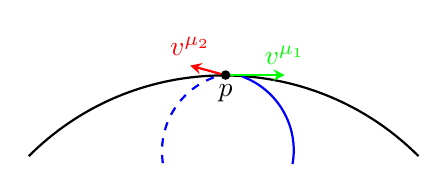
\begin{tikzpicture}[scale=1]
 					\draw [thick] (0,0) arc (45:135:3.5);
 					\draw [thick, blue, dashed] (-2.6, 1) arc (110:190:1);
 					\draw [thick, blue] (-1.6,-0.1) arc (-10:70:1);
 					
 					\draw [->, green, thick, >=stealth] (-2.44, 1.03) -- (-1.7, 1.03) node [above] {$v^{\mu_1}$};
 					\draw [->, red, thick, >=stealth] (-2.46, 1.03) -- (-2.9, 1.15) node [above] {$v^{\mu_2}$};
 					
 					\filldraw (-2.45,1.03) circle (1.5pt) node [below] {$p$};
 				\end{tikzpicture}
 				\caption{An arbitrary 3D curved manifold with a point. A single curve is shown crossing the point along the manifold in blue. Consider the black curvature over the manifold as another curve crossing the point over the manifold. The tangent vector $v^{\mu_1}$ corresponds to the black curve whereas $v^{\mu_2}$ corresponds to the blue curve.}
 			\end{minipage}
 			\hfill
 			\begin{minipage}{0.56\textwidth}
 				\begin{spacing}{1.5}
 					Consider some curved manifold $M$ such that we can parametrize curves that go through some point $p$ on $M$. To define a tangent vector at such a point, recall equation (\ref{eq:TangetVectorWorldline}):
 					$$ v^\mu = \frac{\partial x^\mu}{\partial \lambda}$$
 					We would not like to extend the notion of a tangent vector to all possible worldlines on an arbitrary manifold given a point such that we may obtain a set of all possible tangent vectors represented at this point.
 				\end{spacing}
 			\end{minipage}
 		\end{figure}
 		\vspace{-1cm}
 		\begin{defn}
 			The \textbf{tangent space} for some point $p$ in a $D$-dimensional manifold $M$ is a vector space denoted as the set of all tangent vectors spanned by all the possible curves that intersect $p \in M$, and is denoted $T_p (M)$.
 		\end{defn}
 			\begin{figure}[h]
 				\begin{minipage}{0.4\textwidth}
 					\center
 					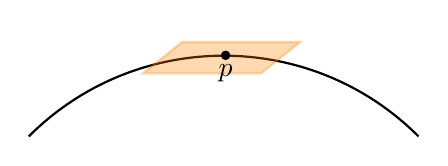
\begin{tikzpicture}[scale=1]
 						\draw [thick] (0,0) arc (45:135:3.5);
 					%	\draw [thick, blue, dashed] (-2.6, 1) arc (110:190:1);
 					%	\draw [thick, blue] (-1.6,-0.1) arc (-10:70:1);
 						
 						\filldraw [thick, orange, opacity=0.3] (-3.0, 1.2) -- (-1.5, 1.2) -- (-2, 0.8) -- (-3.5, 0.8) -- (-3, 1.2); 
 						
 						\filldraw (-2.45,1.03) circle (1.5pt) node [below=] {$p$};
 					\end{tikzpicture}
 					\caption{A tangent space represented as a plane on a point over some 3D manifold.}
 				\end{minipage}
 				\hfill
 				\begin{minipage}{0.54\textwidth}
 					\begin{spacing}{1.5}
 						A tangent vector as we have defined is an example of a vector that is defined for every point on a curve in a manifold. More generally, a tangent vector is a vector that is attached to every point $p \in M$.
 					\end{spacing}
 				\end{minipage}
 			\end{figure}
 			\vspace{-0.5cm}
 			\begin{defn}
 				A \textbf{vector field} is the set of all vectors defined for every point in a manifold $M$. As such, a vector field at some point $p\in M$ is itself a vector.
 			\end{defn}
 			We can think of vectors in many ways, particularly in geometric ones. For instance, vectors can represent differential operators. 
 			\begin{defn}
 				Consider a scalar function over some coordinates given by $a(x^\mu)$ and a tangent vector over the same coordinates $v^{\mu} (x^\mu)$. The \textbf{differential operator}, otherwise known as the \textbf{directional derivative} $v$ is a scalar function such that
 				\begin{equation}
 					\label{eq:DifferentialOperator}
 					\boxed{va = v^{\mu} \frac{\partial}{\partial x^\mu} a = v^\mu a_\mu}
 				\end{equation}
 			\end{defn}
 			Clearly, we have that $a_\mu = \frac{\partial a}{\partial x^\mu} = \partial_\mu a$. It may also be clear that the we are yielding a scalar, or a (0,0)-tensor. To see this, let us write $v$ using the chain rule for a change of coordinates.
 			\begin{align*}
 				v a(x^\mu) &= v^{\mu'} \frac{\partial a (x^\mu)}{\partial x^{\mu'}} \\
 				&= v^{\mu} \left(\frac{\partial x^{\mu'}}{\partial x^\mu}\right) \left(\frac{\partial x^{\nu}}{\partial x^{\mu'}}\right) \frac{\partial a(x^{\mu})}{\partial x^\nu} \\
 				&= \left( \sum_{\mu=0}^{D-1} v^{\mu} \left(\frac{\partial x^{\mu'}}{\partial x^\mu}\right) \right) \left( \sum_{\nu=0}^{D-1} \left(\frac{\partial x^{\nu}}{\partial x^{\mu'}}\right)  \frac{\partial a(x^{\mu})}{\partial x^\nu} \right)
 			\end{align*}
 			We have two different Jacobians: The first $\frac{\partial x^{\mu'}}{\partial x^\mu}$ is for changing from $x^\mu$ to $x^{\mu'}$ coordinates, and the second $\frac{\partial x^{\mu}}{\partial x^{\mu'}}$ is for changing from $x^{\mu'}$ to $x^\mu$ coordinates. They each are respective inverses of the other, and multiplied they yield an identity matrix.
 			
 			\begin{defn}
 				The \textbf{Kronecker delta} is defined as a (1,1)-tensor yielded by the multiplication of a Jacobian by it's own inverse, namely
 				\begin{equation}
 					\label{eq:KroneckerDelta}
 					\boxed{\delta_{\mu}^\nu = \frac{\partial x^{\mu'}}{\partial x^\mu}\frac{\partial x^{\nu}}{\partial x^{\mu'}} = \begin{cases}
 							1, & \text{if } \mu = \nu \\
 							0, & \text{if } \mu \neq \nu \\
 					\end{cases}}
 				\end{equation}
 			\end{defn}
 		
 			The fact that a Jacobian times its inverse results in the Kronecker delta implies that the differential operator on a scalar function becomes
 			$$ va = v^\mu \delta_\mu^\nu \frac{\partial a}{\partial x^\mu} = v^\mu \frac{\partial a}{\partial x^\mu}$$
 			Clearly, this means that this differential operator $v$ transforms a scalar to a scalar. More explicitly, it transforms a (0,0)-Tensor into another (0,0)-Tensor. In calculus terms, it yields the directional derivative of a scalar in the direction of $v$.
 			
 			\begin{exmp}
 				\textbf{A scalar function on a tangent vector}
 				\begin{figure}[h]
 					\begin{minipage}{0.4\textwidth}
 						\center
 						\begin{tikzpicture}[scale=1]
 							%\draw (2,2) node []{$\M$} ;
 							\draw [step=0.5cm, grey, opacity=0.25] (-2.5,-2.5) grid (2.5,2.5);
 							
 							\draw [->] (-2, -2.5) -- (-2, 2) node (taxis) [above] {$t$};
 							\draw [->] (-2.5, -2) -- (2, -2) node (xaxis) [right] {$x$};
 							%\draw [thick, dashed, green] (-2,-2) -- (2.5, 2.5) node [below=20mm, left=5mm] {$\Delta s^2 = 0$};
 							
 							\draw [thick, blue] plot [smooth] coordinates{(-2,-2) (0, 1)  (-1, 2)} (-0.6, 0.3) node [below=5mm] {$\lambda$};
 							\draw [->, thick, red , >=stealth] (0, 1) -- (0.6, 2) node [above =0mm, left=0mm] {$\frac{\partial x^\mu}{\partial \lambda}$};
 							
 							
 							\filldraw (-2, -2) circle (2pt) (-1,2) circle (2pt);
 						\end{tikzpicture}
 						\caption{A worldline on a spacetime manifold parametrized over some coordinate system as $x^{\mu} (\lambda)$, marked in blue. It's tangent vector at some point is marked in red, labelled $\frac{\partial x^\mu}{\partial \lambda}$.}
 					\end{minipage}
 					\begin{minipage}{0.56\textwidth}
 						\begin{spacing}{1.5}
 							Considering a worldline over some manifold $M$, we define a scalar function over the coordinates such that
 							$$ a\big(x^\mu (\lambda)\big) = a(\lambda)$$
 							By the chain rule, the directional derivative on the scalar $a$ is hence given by
 							\vspace{0cm}
 							\begin{align*}
 								\frac{da}{d\lambda} &= \frac{\partial x^\mu}{\partial \lambda} \frac{\partial a}{\partial x^\mu} \\
 								&= v^\mu \frac{\partial}{\partial x^\mu} a \\
 								&=v a
 							\end{align*}
 						\end{spacing}
 					\end{minipage}
 				\end{figure}
 			
 				\vspace{-0.5cm}\noindent
 				This leads us to see that the differential operator $v$ takes derivatives along a curve to which the vector $v^\mu$ is a tangent vector. Sometimes, we might think of $\partial_\mu$ as a \textit{basis} for the tangent vectors $v^\mu$. Thus, a directional derivative is neatly given by a tangential component and a basis component:
 				$$ v = v^\mu \partial_\mu$$
 			\end{exmp}
 			\begin{exe}
 				Consider the manifold $M = \R^2$ in both Cartesian $(x,y)$ and Polar coordinates $(r, \theta)$ such that a tangential vector in Cartesian coordinates is given by
 				$$ v^\mu = \begin{pmatrix}
 					1 \\ 0
 				\end{pmatrix}$$
 			\begin{enumerate}[(a)]
 				\item Write the tangential vector $v^{\mu}$ in polar coordinates.
 				\item Write the differential operator $\frac{\partial}{\partial x^\mu}$ in Polar coordinates.
 				\item Explain how (a) and (b) relate to each other.
 			\end{enumerate}
 			\end{exe}
 			\begin{thm}
 				The tangential vectors $v^\mu$ of a vector $\vec{v}$ on some basis $\frac{\partial}{\partial x^\mu}$ transform from coordinates $x^\mu$ to coordinates $x^{\mu'}$ as
 				$$ v^\mu \to v^{\mu'} = \frac{\partial x^{\mu'} }{\partial x^\mu} v^\mu$$
 				Where $x^{\mu'} = x^{\mu'} (x^\mu)$ and $\frac{\partial x^{\mu'} }{\partial x^\mu}$ is the Jacobian from $x^\mu$ to $x^{\mu'}$.
 			\end{thm}
 			We can therefore represent tangential vectors $v^\mu$ in a coordinate independent way as a differential operator which takes scalars to scalars. Now, let's introduce our next tensor.
 			
 			\begin{defn}
 				Given a $D$-dimensional manifold $M$, a \textbf{one-form} is a (0,1)-tensor given as a set of $D$ functions on some coordinates $x^\mu$ denoted by $w_\mu$. It is otherwise known as \textbf{covariant vector}.
 			\end{defn}
 			\begin{thm}
 				A one form $w_\mu$ on some coordinates $x^\mu$ transforms as
 				$$ w_\mu \to w_{\mu'} = \frac{\partial x^\mu}{\partial x^{\mu'}} w_\mu$$
 			\end{thm}
 			\begin{cor}
 				Given two coordinates $x^\mu$ and $x^{\mu'}$ on a $D$-dimensional manifold $M$, the Jacobian $\frac{\partial x^\nu}{\partial x^{\mu'}}$ that transforms a one form as $w_\nu \to w_{\mu'} = \frac{\partial x^\nu}{\partial x^{\mu'}} w_\nu$ is the inverse of the Jacobian $\frac{\partial x^{\mu'}}{\partial x^\mu}$ that transforms the components of a vector as $v^\mu \to v^{\mu'} = \frac{\partial x^{\mu'}}{\partial x^\mu} v^\mu$ such that
 				$$ \frac{\partial x^{\mu'}}{\partial x^\mu}\frac{\partial x^\nu}{\partial x^{\mu'}} = \delta_{\mu}^\nu$$
 			\end{cor}\noindent
 			The difference between a vector and a one form is that a vector can be represented by contravariant components $v^\mu$ whereas a one-form is represented by covariant components $w_\mu$. Moreover, this extends to why the Jacobians are written in each way respectively for a one form $w_\mu$ and a vector $v^\mu$, as we may get a scalar by summing the multiplication of each function as $v^\mu w_\mu = a$. To show this, let us change from coordinates $x^\mu$ to coordinates $x^{\mu'}$ with the following transformation
 			$$ v^\mu w_\mu \to v^{\mu'} w_{\mu'} = \left( v^\mu \frac{\partial x^{\mu'}}{\partial x^\mu}  \right) \left(\frac{\partial x^\nu}{\partial x^{\mu'}} w_\nu \right)$$
 			By Corollary 2.10, we have
 			$$  v^{\mu'} w_{\mu'} = v^\mu \delta_\mu^\nu w_\nu = v^\mu w_\mu$$
 			\begin{defn}
 				The product of a one-form $w_\mu$ and a vector $v^\mu$ is known as a \textbf{dot-product}.
 			\end{defn}
 			
 			So formally, we can think that a one form $w_\mu$ is a linear mapping from vector components $v^\mu$ to scalars $a$. For this very reason, sometimes one-forms can be referred to as \textit{dual-vectors} that mirror vectors. In the same way a vector belongs to some tangent space, a one form also belongs to a \textit{dual-tangent space} or \textit{cotangent space} denoted $T_{p}^*(M)$. However, this language is saved for much more mathematical formulations of General Relativity. The mention of this vocabulary is done for the sake of reference for further insight into other texts. 
 			
 			In linear algebra, we usually represent vectors as column vectors and one-forms as row vectors. In particular, considering a $D$-dimensional manifold $M$ we have
 			$$ w_\mu = \begin{pmatrix} w_0 & w_1 & \dots & w_{D-1}\end{pmatrix} \quad v^\mu = \begin{pmatrix}
 				v^1 \\
 				v^2 \\
 				\vdots \\
 				v^{D-1}
 			\end{pmatrix} \implies  w_\mu v^\mu = \sum_{\nu=0}^{D-1} w_\nu v^\nu$$
 			Whether a tensor has a covariant (lower) or contravariant (upper) index will impact how that specific tensor transforms under a coordinate change. If we instead have $v^\mu w_\mu$ we would get a $3\times3$ matrix but would only sum the trace of this matrix, yielding the same result as $w_\mu v^\mu$.
 			
 			\begin{defn}
 				Whenever we set a covariant and a contravariant index as equal in a tensor and subsequently sum over them, we denote that as \textbf{contraction of indices}.
 			\end{defn}
 			\begin{thm}
 				For some scalar function $a=a(x^\mu)$ on a $D$-dimensional manifold $M$ given some coordinates $x^\mu$, we can define a one-form $w_\mu$ whose componets are given by
 				\begin{equation}
 					\label{eq:OneForm}
 					\boxed{\frac{\partial a}{\partial x^\mu} = \partial_\mu a}
 				\end{equation}
 			\end{thm} \noindent
 			Now let us change the components of a one-form $w_\mu$ from coordinates $x^\mu$ to coordinates $x^{\mu'}$, we use the chain rule to get
 			$$ \partial_\mu a \to \partial_{\mu'} a = \frac{\partial x^\mu}{\partial x^{\mu'}} \frac{\partial a(x^\mu)}{\partial x^\mu} $$
 			And just like we write vectors using a basis independent way $\vec{v} = v^\mu \partial_\mu$, we can write a one-form in a basis independent way such that
 			$$ w = w_\mu dx^\mu$$
 			\begin{defn}
 				We denote $dx^\mu$ as an \textbf{infinitesimally small displacement of coordinates} $x^\mu$.
 			\end{defn} \noindent
 			Given another set of coordinates $x^{\mu'}$ we can obtain a one form in $x^\mu$ coordinates as
 			$$ w = w_\mu dx^\mu = \left( w_{\mu'} \frac{\partial x^{\mu'}}{\partial x^\mu} \right) \left( \frac{\partial x^\mu}{\partial x^{\nu'}} dx^{\nu'} \right)$$
 			By Corollary 2.10, we again have $\delta_\mu^{\mu'}$, which gives
 			$$ w = w_\mu dx^\mu = w_{\mu'} dx^{\mu'}  $$
 			
 			Now, let us go back to Theorem 2.11 from which we see that for some coordinates $x^\mu$, there exists a special notation for the one-form $w_\mu = \partial_\mu a$, whose components are the derivatives of some scalar function $a=a(x^\mu)$. This notation is called \textbf{integration} of $a$ and is denoted
 			\begin{equation}
 				\label{eq:TheDifferential}
 				\boxed{da = \partial_\mu a \,dx^\mu}
 			\end{equation}
 			\begin{exmp}
 				\textbf{One-form of a Cartesian manifold} \\
 				Consider the $\R^2$ manifold. Let us define a Cartesian coordinate system such that we can define the scalar functions
 				\begin{align*}
 					a(x^1) &= x^1 = x \\
 					a(x^2) &= x^2 = y
 				\end{align*}
 				We can easily obtain the components of the one-form:
 				\begin{align*}
 					\partial_1 a(x^1) &= \begin{pmatrix} 1 & 0 \end{pmatrix} \\
 					\partial_2 a(x^2) &= \begin{pmatrix} 0 & 1 \end{pmatrix}
 				\end{align*} 
 				Therefore, the infinitesimal displacement for each respective component in the one-form will be given by
 				\begin{align*}
 					\partial_1 a(x^1) dx^1 &= \begin{pmatrix} dx & 0 \end{pmatrix} \\
 					\partial_2 a(x^2) dx^2 &= \begin{pmatrix} 0 & dy \end{pmatrix}
 				\end{align*}
 			\end{exmp} \noindent
 			The one-form can be more easily explained as the sum of the derivatives of each coordinate. It yields an independent basis in the same way that the basis for a vector $\frac{\partial}{\partial x^\mu} = \partial_\mu$ does. We can say as physicists that a one-form's one and only purpose is to be integrated such that
 			$$ \int da $$
 		
 		\pagebreak
 			\begin{thm}
 				The \textbf{Fundamental Theorem of Calculus} states that, given two points $p$ and $q$ defined on a function $f$, it follows that
 				\begin{equation}
 					\label{eq:TheoremCalculus}
 					\boxed{\int_p^q df = f(q) - f(p)}
 				\end{equation}
 			\end{thm}
 			We now have enough insight into some basic tensors to generalize and define it formally. Definition 2.6 does provide us with some useful information, but we had to define more things along the way in order to understand what we meant better. Hence, now let us define it using everything we've learned thus far.
 			\begin{defn}
 				A $(k,\ell)$-tensor is a set of $D^{k+\ell}$ functions denoted by
 				$$ T_{\nu_1, \dots, \nu_\ell}^{\mu_1, \dots, \mu_k} = \left( \frac{\partial x^{\mu_{1'}}}{\partial x^{\mu_1}} \right) \cdots \left( \frac{\partial x^{\mu_k'}}{\partial x^{\mu_k}} \right)\left( \frac{\partial x^{\nu_1}}{\partial x^{\nu_{1'}}} \right) \cdots \left( \frac{\partial x^{\nu_\ell}}{\partial x^{\nu_{\ell'}}} \right) $$
 			\end{defn}
 			This looks quite complicated. So we need only remember index contraction such that this eventually simplified. It therefore extremely important to note the ordering and placement of the indices, as changing either will inevitably change the entire tensor. On a last note, we can also write a tensor using a tensor product.
 			By use of the tensor product $T \otimes T'$, a tensor becomes much easier to write down in a coordinate invariant way via contraction of indices.
 			$$ T = T_{\nu_1, \dots, \nu_\ell}^{\mu_1, \dots, \mu_k} \,\,  \partial_{\mu_1} \otimes \cdots \otimes \partial_{\mu_k} \otimes dx^{\nu_1} \otimes \cdots \otimes dx^{\nu_\ell} $$
 			Let us clean this up further. We clearly see that this involves the outer product of several vector spaces, whose elements are vectors, and several dual vector spaces, whose elements are one-forms. Hence, let us define $V_{\mu_i}$ as the vector space for the basis $\partial_{\mu_i}$ where $i=1,\dots, k$ and let us define the dual vector space $W^{\nu_j}$ for the infinitesimal displacement $dx^{\nu_j}$ where $j=1,\dots, \ell$. We can then say that
 			$$T = T_{\nu_1, \dots, \nu_\ell}^{\mu_1, \dots, \mu_k} = V^{\mu_1} \otimes \cdots \otimes V^{\mu_k} \otimes W_{\nu_1} \otimes \cdots \otimes W_{\nu_\ell} $$
 			Moreover, let us give a special notation for the outer product of several vector spaces:
 			$$ V^1 \otimes \cdots \otimes V^n = V^{\otimes_{n}}$$
 			Finally, a tensor can be written in terms of vector spaces and dual vector spaces as
 			$$T = T_{\nu_1, \dots, \nu_\ell}^{\mu_1, \dots, \mu_k}= V^{\otimes_{\mu_k}} \otimes W_{\otimes_{\nu_\ell}} $$
 			
 			\pagebreak
 			
 			\begin{exmp}
 				\textbf{The metric tensor}\\
 				Consider the (0,2)-tensor that denotes the variations of a spacetime metric $g_{\mu\nu}$. We can write this tensor as
 				\begin{equation}
 					\label{eq:MetricTensor}
 					\boxed{g = g_{\mu\nu} dx^\mu \otimes dx^\nu = g_{\mu \nu} dx^\mu dx^\nu}
 				\end{equation}
 			\end{exmp}
 			We have the following operations on tensors:
 			\begin{itemize}
 				\item \textbf{Addition}
 					\subitem Two tensors of the same weight $A_{\nu_1, \dots, \nu_\ell}^{\mu_1, \dots, \mu_k}$ and $B_{\nu_1, \dots, \nu_\ell}^{\mu_1, \dots, \mu_k}$ can be added to obtain another tensor of the same weight $C_{\nu_1, \dots, \nu_\ell}^{\mu_1, \dots, \mu_k}$. To achieve this, we simply add the components of each vector correspondingly to the indices such that we get
 					$$ A_{\nu_1, \dots, \nu_\ell}^{\mu_1, \dots, \mu_k} + B_{\nu_1, \dots, \nu_\ell}^{\mu_1, \dots, \mu_k} = C_{\nu_1, \dots, \nu_\ell}^{\mu_1, \dots, \mu_k}$$
 				\item \textbf{Multiplication}
 					\subitem We can multiply a $(k, \ell)$-tensor $A_{\nu_1, \dots, \nu_\ell}^{\mu_1, \dots, \mu_k}$ with a $(k', \ell')$-tensor $B_{\nu_1, \dots, \nu_{\ell'}}^{\mu_1, \dots, \mu_{k'}}$  to get another\\$(k+k',\ell + \ell')$-tensor $C_{\nu_1, \dots, \nu_{\ell+\ell'}}^{\mu_1, \dots, \mu_{k+k'}}$. So a tensor transforms as a tensor under multiplication, namely
 					$$ A_{\nu_1, \dots, \nu_\ell}^{\mu_1, \dots, \mu_k}\otimes B_{\nu_1, \dots, \nu_{\ell'}}^{\mu_1, \dots, \mu_{k'}} = C_{\nu_1, \dots, \nu_{\ell+\ell'}}^{\mu_1, \dots, \mu_{k+k'}}$$
 				\item \textbf{Contraction}
 					\subitem Given a $(k, \ell)$-tensor $A_{\nu_1, \dots, \nu_\ell}^{\mu_1, \dots, \mu_k}$, we can contract covariant and contravariant indices to get a \\$(k-1, \ell-1)$-tensor  $B_{\nu_1, \dots, \nu_{\ell-1}}^{\mu_1, \dots, \mu_{k-1}}$
 					For instance, $v^\mu w_\nu$ is a (1,1)-tensor while $v^\mu w_\mu$ is a $(0,0)$-tensor.
 			\end{itemize}
 			\begin{exe}
 				Consider the manifold $\R^2$ in coordinates $x^\mu = (x,y)$ and $x^{\mu'} = (r, \theta)$. Given the following tangent vector and the one form in $x^\mu$ coordinates $$ v^\mu = \begin{pmatrix}
 					1 \\ 0
 				\end{pmatrix}, \quad\quad w_\mu = \begin{pmatrix}
 				1 & 0
 			\end{pmatrix}$$
 				\begin{enumerate}[(a)]
 					\item Find the tangent vector $v^{\mu'}$ and the one-form $w_{\mu'}$ in $x^{\mu'}$ coordinates.
 					\item Represent $v = v^\mu \partial_\mu$ and $w = w_\mu dx^\mu$ in coordinate-free notation.
 				\end{enumerate}
 			\end{exe}
 		\pagebreak
 		
 		\subsection{Geometry of Spacetime}
 			We have learned thus far that a tensor is a generalization of scalars, vectors, and matrices such that we denote them by a Cartesian product $(k, \ell)$ of the number of $k$ contravariant and $\ell$ covariant indices in the tensor to yield its rank $r=k+\ell$. Thus, a $(k, \ell)$-tensor on a $D$-dimensional manifold $M$ is a set of $D^{r}$ functions which transform as
 			$$ T^{\mu_1' \dots \mu_k'}_{\nu_1' \dots \nu_\ell'} = \left( \frac{\partial x^{\mu_1'}}{\partial x^{\mu_1}} \right) \cdots \left( \frac{\partial x^{\mu_k'}}{\partial x^{\mu_k}} \right) \left( \frac{\partial x^{\nu_1}}{\partial x^{\nu_1'}} \right) \cdots \left( \frac{\partial x^{\nu_\ell}}{\partial x^{\nu_\ell'}} \right) = V^{\otimes_{\mu_k'}} \otimes W_{\otimes_{\nu_\ell}}$$
 			Furthermore, a (1,0)-tensor will transform using the contravariant Jacobian $\partial_\mu x^{\mu'}$ while a (0,1)-tensor will transform using the covariant Jacobian $\partial_{\nu'} x^\nu$, which is just the inverse of the contravariant Jacobian. Thus, a $(k, \ell)$-tensor is said to transform using $k$-Jacobians and $\ell$-inverse Jacobians. A contravariant Jacobian will have free indices $\mu'$ in the numerator while it is summed over the dummy indices $\mu$ in the denominator, whereas a covariant Jacobian has free indices $\nu'$ in the denominator and gets summed over the dummy indices $\nu$ in the numerator. So we denote the name for a Jacobian depending on whether the covariant or contravariant indices are free indices. Lastly, the contravariant Jacobians belong to the vector space $\partial_{\mu_k} x^{\mu_k '} \in V^{\otimes_{\mu_k'}}$ while the covariant derivatives belong to the dual-vector space $\partial_{\nu_\ell '} x^{\nu_\ell} \in W_{\otimes_{\nu_\ell}}$
 			
 			We also learned that we have various algebraic operations that can be done on tensors, including tensor addition, tensor multiplication, and index contraction. Respectively, recall an example for each operation:
 			\begin{itemize}
 				\item \textbf{Tensor addition}
 				$$ A^{\alpha\beta\gamma}_{\mu\nu} + B^{\alpha\beta\gamma}_{\mu\nu} = C^{\alpha\beta\gamma}_{\mu\nu}$$
 				So the addition of two $(k,\ell)$-tensors results in another $(k,\ell)$-tensor
 				
 				\item \textbf{Tensor Multiplication}
 				$$ A^{ij}_{\mu\nu} \otimes B^{k\ell}_{\alpha\beta} = C^{ijk\ell}_{\mu\nu\alpha\beta}$$
 				So the tensor product of a $(k, \ell)$ tensor and a $(k', \ell')$ tensor is a $(k+k', \ell+\ell')$-tensor. Note that tensor products do not allow us to define all tensors as the multiplication of arbitrary tensors of lower order. This is only true for special tensors, like Jacobians. 
 				
 				\item \textbf{Index contraction}
 				$$ A^{ij}_{\alpha\beta}w_jv^\beta = fA^{i}_{\alpha\beta}v^\beta = fgA^i_\alpha$$
 				So contraction of indices of a $(k, \ell)$-tensor results in a $(k-n,\ell-m)$-tensor, where $n$ and $m$ are the number of contravariant and covariant indices being contracted from the tensor. Each contraction will result in a scalar, which is what $f$ and $g$ represent.
 				
 			\end{itemize}
 			So notice how our definition of a tensor includes both contraction of indices and tensor multiplication of Jacobians. As noted, multiplication does not generally define higher order tensors, as only Jacobians are able to do so. 
 			
 			\begin{defn}
 				A \textbf{permutation} $\sigma$ of an ordered set of objects is a reordering of the elements of the set without removing any of them. It is a bijective function that maps all elements from a set to a new set with different ordering. We say that $\sigma$ is a product of pairwise interchanges
 			\end{defn}
 			Having defined permutations, we may not consider two additional operations on tensors
 			\begin{itemize}
 				\item \textbf{Symmetrization}
 				\subitem A \textbf{symmetrization} is the sum of all the permutations of the indices of a tensor. Letting $\varsigma$ be the set of all permutations $\sigma = \sigma(\mu_i)$ for $i=1,\dots, \ell$, we have symmetrization given as a parenthesis surrounding the indices such that
 				$$ T_{\left(\mu_1 \dots \mu_\ell\right)} = \frac1{\ell!} \sum_{\sigma \in \varsigma} T_{\sigma(\mu_1) \dots \sigma(\mu_\ell)} $$
 				
 				\item \textbf{Anti-symmetrization}
 				\subitem An \textbf{anti-symmetrization} is the sum of all the permutations of the indices of a tensor including their corresponding sign. Letting $\varsigma$ be the set of all permutations $\sigma = \sigma(\mu_i)$ for $i=1,\dots, \ell$, we have anti-symmetrization given as square brackets surrounding the indices such that
 				$$ T_{\left[\mu_1 \dots \mu_\ell\right]} = \frac1{\ell!} \sum_{\sigma \in \varsigma} \sgn(\sigma) T_{\sigma(\mu_1) \dots \sigma(\mu_\ell)} $$
 				Where
 				$$ \sgn(\sigma) = (-1)^n \for \sigma \in \varsigma$$
 			\end{itemize}
 			\begin{exmp}
 				\textbf{Symmetrization and anti-symmetrization on a tensor}
 				\begin{align*}
 					T^{\left[\mu_1\mu_2\right]}_{\nu_1 \left(\nu_2\nu_3\right)} &= \frac{1}{2} \left( T^{\mu_1 \mu_2}_{\nu_1 \left(\nu_2\nu_3\right)} - T^{\mu_2 \mu_1}_{\nu_1 \left(\nu_2\nu_3\right)} \right) \\
 					&=\frac{1}{2} \left( \frac{1}{2} \left( T^{\mu_1 \mu_2}_{\nu_1\nu_2\nu_3} + T^{\mu_1 \mu_2}_{\nu_1\nu_3\nu_2} \right) -  \frac{1}{2} \left( T^{\mu_2 \mu_1}_{\nu_1\nu_2\nu_3} + T^{\mu_2 \mu_1}_{\nu_1\nu_3\nu_2} \right) \right) \\
 					&= \frac{1}{4} \left(T^{\mu_1 \mu_2}_{\nu_1\nu_2\nu_3} + T^{\mu_1 \mu_2}_{\nu_1\nu_3\nu_2} - T^{\mu_2 \mu_1}_{\nu_1\nu_2\nu_3} - T^{\mu_2 \mu_1}_{\nu_1\nu_3\nu_2} \right)
 				\end{align*}
 			\end{exmp}
 			\begin{lem}
 				An anti-symmetric tensor is one which equals its anti-symmetrization and picks up a change in sign given by $\sgn(\sigma)$. Moreover, if the indices undergoing anti-symmetrization are equal, then anti-symmetrization yields a zero tensor\footnote{Not a (0,0)-tensor, but instead all elements of the tensor are zero}. A symmetric tensor is one which remains invariant over symmetrization.
 			\end{lem}
 			\begin{defn}
 				A \textbf{differential form} of rank $n$ or an \textbf{$n$-form}, is an anti-symmetric $(0,n)$-tensor.
 			\end{defn}
 		\pagebreak
 			We have hence generalized one forms and scalars onto differential forms or $n$-forms. We see that a one-form is indeed an anti-symmetric $(0,1)$-tensor and a scalar is a $(0,0)$-tensor, which by definition is symmetric and anti-symmetric.
 			
 			Let us recall some examples of tensors:
 			\begin{multicols}{2}
 				\begin{itemize}
 					\item Scalars: $f \equiv (0,0)$-tensor
 					\item One-Forms:\\ $w_\mu = \frac{\partial f}{\partial x^\mu}  \equiv (0,1)$-tensor
 					\item Force-field: \\$F_{\mu\nu} = - F_{\nu\mu} \equiv $ antisymmetric $(0,2)$-tensor\footnote{This is known as the electromagnetic field strength tensor where $F_{0i} = E_i$ and $F_{ij} = \varepsilon_{ijk} B_k$.}
 					\item Vectors: $v^\mu = \frac{d x^\mu}{d \lambda} \equiv (1,0)$-tensor
 					\item Kronecker delta: \\
 					$\frac{\partial x^{\mu'}}{\partial x^\nu} \frac{\partial x^\mu}{\partial x^{\mu'}} = \delta^\mu_\nu \equiv (1,1)$-tensor
 					\item Metric tensor:\\
 					$ g_{\mu\nu} \equiv $ symmetric $(0,2)$-tensor
 				\end{itemize}
 			\end{multicols}            
 			Now recall the \hyperref[defn:GeneralCovariance]{Principle of General Covariance} which states that the laws of physics make predictions independently of the chosen coordinate systems for observing these laws. For instance, if we define a certain coordinate system to observe planetary motion, then the laws that govern the motion of the planets should be invariant of coordinate changes. That is, if we define another coordinate system, it will not affect the observed motion of the planets. It will only affect the representation in regards to a new coordinate system.
 			
 			\begin{lem}
 				By the Principle of General Covariance, all laws of physics can be represented through tensors. Moreover, the tensors in the equations must have the same .
 			\end{lem}
 			
 			This means that when we write any physical law in a particular coordinate system, it most follow from a tensor equation of the form
 			$$ T^{\mu_1 \dots \mu_k}_{\nu_1 \dots \nu_\ell} = S^{\mu_1 \dots \mu_k}_{\nu_1 \dots \nu_\ell} $$
 			Where $T$ and $S$ are the tensor representations in the same coordinate system given by their indices. In a new coordinate system, it would take \textit{exactly the same form} because the tensor transformation rule implies we multiply a tensor by its invertible Jacobian.
 			$$ T_{\nu_1' \dots \nu_\ell'}^{\mu_1' \dots \mu_k'} = S_{\nu_1' \dots \nu_\ell'}^{\mu_1' \dots \mu_k'}$$
 			This mirrors the fact that vectors under passive coordinate transformations do not change themselves, but rather their components do. With this, we can further solidify and conclude our understanding of the Principle of General Covariance. 
 
 			Often in physics we tend to write equations of motion as differential equations. However, we do not yet know how to differentiate and take derivatives for a tensor in a \textit{covariant manner}. That is, imagine a vector $v^\mu$ in a $D$-dimensional Manifold given a particular coordinate system $x^\mu$. Recall,
 			$$ v^{\mu} \to \partial_\nu v^\mu $$
 			Take note that this \textbf{is not a (1,1)-tensor}. It acts on a vector which has one contravariant index. We know how to take derivatives for scalars and vectors from vector calculus, but this knowledge cannot be extrapolated to vectors. It turns out that to differentiate on tensors, we require \textit{Riemannean Geometry}. So we need to develop \textit{covariant derivatives} to better understand how differentiation on a tensor would work.
 			
 			Recall the implications of the \hyperref[defn:StrongEquivalence]{Einstein Equivalence Principle} which particularly state that the effect of gravity is, in small reference frames, locally like Minkowski space and equivalent to an accelerating reference frame. Knowing tensors, we can give a more mathematical definition for this principle.
 			\begin{thm}
 				By the Equivalence Principle, we say that spacetime is a manifold with a defined metric $g_{\mu\nu}$ that is defined by the line element
 				
 				\begin{equation}
 					\label{eq:MetricInterval}
 					\boxed{ ds^2 = g_{\mu\nu}dx^\mu dx^\nu}
 				\end{equation}
 				Such that for any point $p\left(x^\mu\right)$, there is a corresponding coordinate system $x^\mu$ such that as $x^\mu \to p$, we have
 				$$ g_{\mu\nu} = \eta_{\mu\nu}$$
 			\end{thm} 
 			We can then assume that a Taylor approximation of the coordinates to this point results in the first term being the metric for flat spacetime. It is not the case that every coordinate can be expanded upon some point to yield flat spacetime however, we are assuming that there exists a coordinate system which can be approximated to flat spacetime at this point. So clearly, $g_{\mu\nu} \neq \eta_{\mu\nu} \quad \forall p \in M$. This means that $g_{\mu\nu}$ is a $(0,2)$-tensor with the following properties:
 			
 			\begin{itemize}
 				\item Symmetric: $g_{\mu\nu} = g_{\nu\mu}$ 
 				\item Invertible: $\det(g_{\mu\nu}) = g \neq 0$
 				\item Diagonalizable: $\det(g_{\mu\nu}-\lambda I) =0\implies\lambda =(-1,+1,+1,+1)$
 			\end{itemize}
 			To show that these properties indeed hold for the metric $g_{\mu\nu}$, we note that there exists a basis where $g_{\mu\nu} = \eta_{\mu\nu}$. Clearly, in any other coordinate system, $g_{\mu\nu}$ will take the form of a set of Jacobians such that
 			$$ g_{\mu\nu} = \left( \frac{\partial x^{\mu'}}{\partial x^\mu} \right)\left( \frac{\partial x^{\nu}}{\partial x^{\nu'}} \right)\eta_{\mu' \nu'} + \dots$$
 			In matrix notation, we would have
 			\begin{equation}
 				\label{eq:MetricMatrix}
 				\boxed{g_{\mu\nu} = \left( \frac{\partial x^{\nu}}{\partial x^{\nu'}} \right)\begin{psmallmatrix}
 						-1 & 0 & 0 & 0 \\
 						0 & +1& 0 & 0 \\
 						0 & 0 & +1 & 0 \\
 						0 & 0 & 0 & +1
 					\end{psmallmatrix}\left( \frac{\partial x^{\mu'}}{\partial x^\mu} \right) = J^T \eta_{\mu'\nu'} J}
 			\end{equation}
 			As expected, we have that $ \frac{\partial x^{\nu}}{\partial x^{\nu'}}  = J$ is the Jacobian in a change of basis and it is also invertible. Note that as long as the matrix between the Jacobians has a nonzero determinant, the resulting metric will be invertible as well. These statements are coordinate invariant as well, so if they are true in one coordinate system, they are true in all coordinate systems. In other words, both $g_{\mu\nu}$ and $\eta_{\mu\nu}$ are symmetric.
 			
 			\begin{defn}
 				A \textbf{metric} is an invertible symmetric (0,2)-tensor.
 			\end{defn}
 			If the eigenvalues of the metric are all positive, then it is considered a \textbf{Riemannian} or \textbf{Euclidean} metric, otherwise it is denoted as a \textbf{pseudo-Riemannian} or \textbf{Lorentzian} metric. Furthermore, the number of positive and negative eigenvalues of the metric are denoted as the \textbf{metric signature}.
 			
 			\begin{exmp}
 				\textbf{Spacetime in General Relativity}\\
 				In General Relativity, spacetime is a pseudo-Riemannian metric of signature (-,+,+,+), or (1,3).
 			\end{exmp}
 		
 			We now wish to further develop Riemannian and pseudo-Riemannian geometry for the sake of better understanding General Relativity. Recall that spacetime is a manifold that comes along with a metric, which is an invertible (0,2)-tensor.
 			\begin{defn}
 				The \textbf{inverse of the metric} $g_{\mu\nu}$ is denoted $g^{\mu\nu}$, which is a symmetric (2,0)-tensor.
 			\end{defn} \noindent
 			In order to understand why this is indeed a (2,0)-tensor, we see that
 			\begin{equation}
 				\label{eq:MetricIdentity}
 				\boxed{g^{\mu\nu}g_{\nu\rho} = \delta_\rho^\mu} \quad\quad \text{OR} \quad\quad \boxed{g_{\mu\nu}g^{\nu\rho} = \delta_\mu^\rho}
 			\end{equation}
 			Where $\delta_\rho^\mu$ is the identity matrix of the size of the metric. We now use $g_{\mu\nu}$ and $g^{\mu\nu}$ to raise and lower indices by Einstein summation notation. Given a vector $v^\mu$, we define a one-form $v_\mu = g_{\mu\nu}v^\mu$. Hence, we sum over the free indices of the vector. Similarly, given a one-form $w_\mu$, we define a vector $w^\mu = g^{\mu\nu} w_\nu$. So for a tensor, for instance a (2,1)-tensor, we have
 			$$T^{\mu\nu}_{\rho} = g_{\rho \sigma} T^{\mu\nu\sigma} \quad\quad \text{OR} \quad\quad T^{\mu\nu}_{\,\,\,\,\rho} = g_{\rho\sigma} T^{\mu\sigma\nu}$$
 			\begin{defn}
 				The \textbf{norm} of a vector $v^\mu$ and a one-form $w_\mu$ are respectively given by
 				$$ v^2 = v_\mu v^\mu \quad \quad \text{AND} \quad \quad w^2 = w_\mu w^\mu$$
 			\end{defn} \noindent
 			We can the define whether a vector is space-like, time-like, or null-like from the value of $v^2$. In our signature, 
 			\begin{align*}
 				v^2 > 0 &\implies v \text{ is space-like}\\
 				v^2 < 0 &\implies v \text{ is time-like}\\
 				v^2 = 0 &\implies v \text{ is null-like}
 			\end{align*}
 		\pagebreak
 			\begin{exe}
 				Consider the manifold $\R^2$ with two different coordinate systems $x^\mu = (x,y)$ and $x^{\mu'} = (r, \theta)$. We have some curve given by $(x,y) = R (cos\lambda, sin \lambda)$, where $\lambda$ is the parametrization on the curve and $R$ is a rotation matrix. Compute in both $x^\mu$ and $x^{\mu'}$
 				\begin{enumerate}[$\quad\quad$(a)]
 					\item $v^{\mu} = \dot{x}^\mu = \frac{dx^\mu}{d\lambda}$
 					\item $v_\mu$
 					\item $v_\mu v^\mu$
 				\end{enumerate}
 			\end{exe}
 			
 			So far, we have seen that spacetime is a manifold with a $(0,2)$ symmetric tensor $g_{\mu\nu}$ which determines the line element
 			$$ ds^2 = g_{\mu\nu} dx^\mu dx^\nu$$
 			Where the line element $ds^2$ is what we use to determine invariant intervals. Locally, spacetime looks like Minkowski space by the Principle of general covariance. The idea is that the metric $g_{\mu\nu}$ determines the geometry of spacetime in the sense that it allows us to determine the invariant interval between points in spacetime, and also the length of paths through spacetime. 
 			
 			Given a $D$-dimensional manifold $M$, we define a worldline $x^\mu(\lambda)$ as a set of $D$ functions of the parameter $\lambda$ measuring where we are on the worldline. Thus, $\lambda$ will label different points along the worldline through spacetime. The way in which we determine the length of some worldline in spacetime is by writing the similar integration of invariant intervals as would be done in Special Relativity.
 			\begin{equation}
 				\label{eq:DefiniteInterval}
 				\boxed{S = \int_{\lambda_0}^{\lambda_1} ds 
 				= \int_{\lambda_0}^{\lambda_1} \sqrt{g_{\mu\nu} \dot{x}^\mu \dot{x}^\nu} d\lambda}
 			\end{equation}
 			Where $\dot{x}^\mu = \frac{dx^\mu}{d\lambda}$ is the tangent vector to the worldline.
 			\begin{defn}
 				We say that $S$ is the \textbf{interval} or \textbf{proper distance} connecting two events $x^\mu (\lambda_0)$ and $x^\mu (\lambda_1)$ in spacetime along a worldline $x^\mu (\lambda)$. In terms of the proper time measured by an observer moving along the worldline in spacetime, we have
 				$$ \tau = iS$$
 			\end{defn}
 			In this sense, the metric determines the geometry of spacetime as we saw above. However, this interval will only apply to a specific worldline. If we instead would like connect any two points in spacetime, we need to define a worldline which extremizes the invariant interval between two points.
 			\begin{defn}
 				A worldline which extremizes the interval $ S\left[ x^\mu (\lambda) \right]$ is called a \textbf{geodesic}. The \textbf{geodesic distance} is the length of a geodesic between two events $x^\mu (\lambda_0)$ and $x^\mu (\lambda_1)$.
 			\end{defn} 
 			As in Special Relativity, we have 3 cases for classifying geodesics.
 			\begin{align*}
 				S \in \R &\implies x^\mu(\lambda) \text{ is space-like}\\
 				S \in \C &\implies x^\mu(\lambda) \text{ is time-like}\\
 				S = 0 &\implies x^\mu(\lambda) \text{ is null-like}
 			\end{align*}
 			So the metric will yield the geodesic distance, that is, the geometric distance of two events in spacetime. By geometry, we simply mean the study of distance between points on a manifold. So the question arises on how a geodesic might look like. 
 			
 			We begin by considering the invariant interval between two events as measured along some worldline as
 			\begin{equation}
 				\label{eq:IntervalWorldlineGR}
 				\boxed{S \left[ x^\mu (\lambda) \right] = \int \sqrt{g_{\mu\nu} \dot{x}^\mu \dot{x}^\nu} d\lambda}
 			\end{equation}
 			Where the integrand is 
 			$$\sqrt{g_{\mu\nu} \dot{x}^\mu \dot{x}^\nu} = \frac{ds}{d\lambda}$$
 			What we mean by extremizing is that if we were to change the worldline by a small amount such that
 			$$ x^\mu \to x^\mu + \delta x^\mu$$
 			We essentially demand that the variation on the interval vanishes as $\delta S=0$. This is the same as the action seen in Classical Mechanics. Recall that the principle of least action states that the action can be minimized such that the integrand is given by the equations of motion which we denote as the \textbf{Euler-Lagrange equations}. Hence,
 			\begin{equation}
 				\label{eq:2.17}
 				\boxed{0 = \frac{\delta S}{\delta x^\mu} = \frac{d}{d\lambda} \left( \frac{g_{\mu\alpha} \dot{x}^\alpha}{\sqrt{g_{\mu\nu} \dot{x}^\mu \dot{x}^\nu}} \right) - \frac12 \left( \frac{\partial g_{\alpha\beta}}{\partial x^\mu}\frac{ \dot{x}^\alpha\dot{x}^\beta}{\sqrt{g_{\mu\nu} \dot{x}^\mu \dot{x}^\nu}}\right)}
 			\end{equation}
 			In Classical Mechanics, we consider a particle moving through space as a function of time such that
 			$$ S \left[ x^i (t)\right] = \int dt \Lgr \left( x^i, \dot{x}^i \right)\implies \frac{d}{dt} \left( \frac{\partial \Lgr}{\partial \dot{x}^i}\right) - \frac{\partial \Lgr}{\partial x^i} = 0$$
 			So in General Relativity, considering $\dot{x}^\mu = \frac{d x^\mu}{d\lambda}$, we have
 			\begin{align*}
 				0 &= -g_{\mu\alpha} \dot{x}^\alpha \frac{\left(\nicefrac{d^2s}{d\lambda^2}\right)}{\left(\nicefrac{ds}{d\lambda}\right)^2} + \frac{1}{\nicefrac{ds}{d\lambda}} \left( g_{\mu \alpha} \ddot{x}^\alpha + \left(\frac{\partial g_{\mu\alpha}}{\partial x^\beta} - \frac12 \frac{\partial g_{\alpha \beta}}{\partial x^\mu} \right)\dot{x}^\alpha \dot{x}^\beta \right)  \\
 				&= -g_{\mu\alpha} \dot{x}^\alpha \frac{\left(\nicefrac{d^2s}{d\lambda^2}\right)}{\left(\nicefrac{ds}{d\lambda}\right)^2} + \frac{1}{\nicefrac{ds}{d\lambda}} \left( g_{\mu \alpha} \ddot{x}^\alpha + \frac12\left(\frac{\partial g_{\mu\alpha}}{\partial x^\beta} +\frac{\partial g_{\mu\beta}}{\partial x^\alpha} -  \frac{\partial g_{\alpha \beta}}{\partial x^\mu} \right)\dot{x}^\alpha \dot{x}^\beta\right) \\
 				&= -g_{\mu\alpha} \dot{x}^\alpha \frac{\left(\nicefrac{d^2s}{d\lambda^2}\right)}{\left(\nicefrac{ds}{d\lambda}\right)^2} + \frac{1}{\nicefrac{ds}{d\lambda}} \left( g_{\mu \alpha} \ddot{x}^\alpha + g_{\mu\alpha} \dot{x}^\alpha \left(\frac{\nicefrac{d^2s}{d\lambda^2}}{\nicefrac{ds}{d\lambda}}\right)\right)
 			\end{align*}
 			Considering the parenthesis only, we now multiply everything inside it by the inverse metric $g^{\nu\mu}$ to get
 			\begin{equation}
 				\label{eq:GeodesicEquation}
 				\boxed{\ddot{x}^\nu + \Gamma^\nu_{\alpha\beta} \,\, \dot{x}^\alpha \dot{x}^\beta = \dot{x}^\nu \left(\frac{\nicefrac{d^2s}{d\lambda^2}}{\nicefrac{ds}{d\lambda}}\right)}
 			\end{equation}
 			This is called the \textbf{Geodesic equation} which is a differential equation obeyed by a worldline that extremizes the distance between two events in spacetime.
 			\begin{defn}
 				A \textbf{Christoffel symbol} or \textit{connection in a metric} is defined as 
 				\begin{equation}
 					\label{eq:ChristoffelSymbol}
 					\boxed{
 						\Gamma_{\alpha\beta}^\nu \equiv \frac12 g^{\mu\nu} \left( \frac{\partial g_{\alpha\mu}}{\partial x^\beta} + \frac{\partial g_{\beta\mu}}{\partial x^\alpha} - \frac{\partial g_{\alpha\beta}}{\partial x^\mu} \right)
 					}
 				\end{equation}
 			\end{defn}
 			\noindent
 			An alternative way to write the Geodesic equation in a cleaner way is
 			\begin{equation}
 				\label{eq:CleanGeodesic}
 				\boxed{\ddot{x}^\mu + \Gamma_{\nu\rho}^\mu \,\, \dot{x}^\rho \dot{x}^\nu = f(\lambda) \dot{x}^\mu}
 			\end{equation}
 			We emphasize that it is the order of the indices and not the choice of variable to represent them that matters. Particularly, $\lambda$ is a parameter used to label points along a geodesic. We could always choose a new parameter $\lambda'$ which would be a function of the old parameter $\lambda'(\lambda)$, which then would change the RHS of the geodesic equation. It is always possible to choose a parameter such that the RHS is zero. More explicitly, we have
 			$$ f(\lambda) = \frac{\nicefrac{d^2s}{d\lambda^2}}{\nicefrac{ds}{d\lambda}} $$
 			So we can set $f=0$ using $S$ itself. In other words, we choose $\lambda$ such that as an observer travels along the geodesic through spacetime, the length between the starting point and the ending point is given as
 			$$ S\left(\lambda_0, \lambda \right) = \lambda$$
 			This means that given a starting point $\lambda_0$ and some point along the worldline $\lambda_1$, we can then say that $S\left(\lambda_0, \lambda_1 \right) = \lambda_1$, so $\partial_\lambda S = 1$ and $\partial_{\lambda}^2 S = 0$.
 			\begin{defn}
 				A parametrization variable $\lambda$ that yields $$f(\lambda) = \frac{\nicefrac{d^2s}{d\lambda^2}}{\nicefrac{ds}{d\lambda}}  = 0$$
 				Where $\partial_\lambda S = 1$ and $\partial_{\lambda}^2 S = 0$ is called an \textbf{affine parameter}.
 			\end{defn}
 			For an affine parameter, the geodesic equation takes a particularly simple form given by
 			\begin{equation}
 				\label{eq:AffineGeodesic}
 				\boxed{\ddot{x}^\mu + \Gamma^\mu_{\nu\rho} \dot{x}^\nu \dot{x}^\rho = 0}
 			\end{equation}
 		
 		\pagebreak
 			We note that this definition applies to most cases but not all. Sometimes, using non-affine parameters is far more ideal. An example would be computing the geodesic for a null-like interval, as $S=0$ for any two points on the geodesic, so it would be impossible to chose an affine parameter.
 			
 			Now, recall the Christoffel symbol, but redefined with different ordering of the same indices and with a simpler first partial derivative $\partial_\mu g_{\alpha\beta} = g_{\alpha\beta; \mu}$ such that
 			$$ \Gamma^\mu_{\nu\rho} = \frac12 g^{\mu\sigma} \left( g_{\nu\sigma;\rho} + g_{\rho\sigma;\nu} - g_{\nu\rho;\sigma} \right)$$
 			The Christoffel symbol has various important properties:
 			\begin{itemize}
 				\item Covariant symmetry: $\Gamma_{\nu\rho}^\mu = \Gamma_{\rho\nu}^\mu$
 				\item Not a tensor:
 				\subitem A Christoffel symbol transforms as
 				\begin{equation}
 					\label{eq:ChristoffelTransformation}
 					\boxed{
 						\Gamma_{\nu' \rho'}^{\mu'} = \frac{\partial x^{\mu'}}{\partial x^{\mu}}\frac{\partial x^{\nu}}{\partial x^{\nu'}}\frac{\partial x^{\rho}}{\partial x^{\rho'}} \Gamma_{\nu \rho}^{\mu} - \frac{\partial x^{\rho}}{\partial x^{\rho'}}\frac{\partial x^{\nu}}{\partial x^{\nu'}}\frac{\partial^2 x^{\mu'}}{\partial x^{\rho}\partial x^{\nu}}
 					}
 				\end{equation}
 			\end{itemize}
 		
 			The change of coordinates for a Christoffel symbol involves the second derivative with respect to coordinates, as if it only involved the first derivative then $\ddot{x}^\mu = \ddot{x}^{\mu'} = 0$. In order to get new terms for a change of coordinates on a straight line, we would require second order derivatives to allow for these terms to arise. This reflects the fact that changing from a static coordinate system to an accelerating coordinate system will yield fictitious forces. So equation (\ref{eq:AffineGeodesic}) tells us that, in the case of Minkowski flat spacetime, there will be some fictitious forces in an accelerating coordinate system. So if we have $\ddot{x}^\mu = 0$ then $\ddot{x}^{\mu'} = F_{f}$ where $F_{f}$ are the fictitious forces. This directly mirrors what is achieved in Classical Mechanics when deriving centrifugal forces and gravitational potentials, which are the fictitious forces that arise as from changing from an inertial frame of reference to an accelerating frame of reference. From above, we also note that these forces can be written in terms of the second order derivatives of the spacetime metric $g_{\mu\nu}$.
 			
 			\vspace{0.5cm}
 			The Christoffel symbol $\Gamma_{\nu\rho}^\mu$captures in some sense how geodesics deviate from being "straight lines" with $\ddot{x}^\mu = 0$. We know that a straight line can look very complicated in an accelerating coordinate system, such as Coriolis forces. In the case of General Relativity, we instead consider that these deviations arise from the geometry of spacetime. Particularly, the Christoffel symbol captures the deviation of $\ddot{x}^\mu$ from being equal to zero (ie. a straight line) due to being in an accelerating reference frame and the curvature of spacetime, which is gravitation due to the equivalence principle. Hence, we consider geodesics as curves that are extremized with respect to their distance over curved spacetime.
 			
 			\pagebreak
 			
 			\begin{exmp}
 				\textbf{Geodesics over different surfaces}
 				\begin{figure}[h]
 					\begin{subfigure}{0.46\textwidth}
 						\center
 						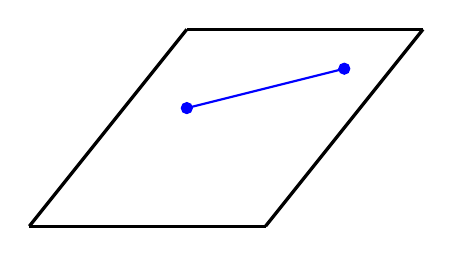
\begin{tikzpicture}
 							\draw [very thick] (-1,-2) -- (1,0.5);
 							\draw [very thick] (2,-2) -- (4,0.5);
 							\draw [very thick] (-1,-2) -- (2,-2);
 							\draw [very thick] (1,0.5) -- (4,0.5);
 							
 							\draw [thick, blue] (1, -0.5) -- (3, 0);
 							
 							\filldraw [blue] (1, -0.5) circle (2pt)
 							(3,0) circle (2pt);
 						\end{tikzpicture}
 						\vspace{0.5cm}
 						\caption{Geodesic over a flat surface}
 					\end{subfigure}
 					\begin{subfigure}{0.46\textwidth}
 						\center
 						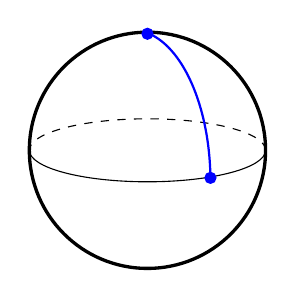
\begin{tikzpicture}
 							\draw [very thick] (0,0) circle (1.5cm);
 							\draw [dashed] (1.5,0) arc (0:180:1.5 and 0.4);
 							\draw (1.5,0) arc (0:180:1.5 and -0.4);
 							
 							\draw [thick, blue] (0.8, -0.35) arc (1.5:80:1 and 1.93);
 							
 							\filldraw [blue] (0.8,-0.35) circle (2pt)
 							(0,1.48) circle (2pt);
 						\end{tikzpicture}
 						\caption{Geodesic over a spherical surface}
 					\end{subfigure}
 					\caption{In the same way that the distance over two points on the surface of a sphere is extremized, yet curved, we can consider the same thing for geodesics over curved spacetime.}
 					
 				\end{figure}
 			
 				As we know that $S \in \C \implies$ time-like geodesic, $S\in \R \implies$ space-like geodesic, and $S = 0 \implies$ null-like geodesic, then it follows that the tangent vector to such a geodesic will be the same, ie. A time-like geodesic will have a time-like tangent vector, and so on.
 			\end{exmp}
 			\begin{exe}
 				Consider the manifold $\R^2$ such that $ds^2 = dx^2 + dy^2 = dr^2 + r^2 d\theta^2$. Compute $\Gamma_{\nu\rho}^\mu$ in both coordinates.
 			\end{exe}
 		\subsection{Calculus of Tensors}
 			We know that spacetime is a manifold with a (0,2) metric tensor $g_{\mu\nu}$, from which we can yield intervals over coordinates using geodesics to extremize the distance between two points in spacetime. The geodesic equation of some worldline defined by the functions $x^\mu (\lambda)$ is given by equation (\ref{eq:CleanGeodesic}), where $\lambda$ is the parametrization variable of the worldline. So the geodesic is a differential equation where $\Gamma_{\nu\rho}^\mu$, as defined in equation (\ref{eq:ChristoffelSymbol}), captures the deviation from $\ddot{x}^\mu = 0$ (ie. a straight line) in terms of both fictitious forces and the curvature of spacetime. Also recall that $\Gamma_{\nu\rho}^\mu$ is not a tensor as it transforms as seen in equation (\ref{eq:ChristoffelTransformation}).
 			
 			The principle of general covariance implies that the laws of physics must be represented through tensors. We also saw that these laws involve derivatives, so we need to learn how to take derivatives of tensors in a way that the derivation yields another tensor. 
 			\begin{exmp}
 				\textbf{Known derivatives}
 				\begin{itemize}
 					\item$\frac{\partial f}{\partial x^\mu} = \partial_\mu f = f_{;\mu} $ is a (0,1)-tensor if $f$ is a $(0,0)$ tensor.
 					\item $\frac{\partial v^\rho}{\partial x^\mu} = \partial_\mu v^\rho = v^\rho_{;\mu}$ is \textbf{not} a (1,1)-tensor even if $v^\rho$ is a (1,0)-tensor.
 				\end{itemize}
 			\end{exmp}
 			The example above shows that we need a new kind of derivative different from our usual partial derivatives $\partial_\mu v^\rho$.
 			\begin{defn}
 				A \textbf{covariant derivative} is denoted $\Del_\mu$ such that
 				$\Del_\mu v^\rho$ is a $(1,1)$-tensor. 
 			\end{defn}
 		\pagebreak
 			\begin{exmp}
 				\textbf{Covariant derivatives of scalars}
 				\begin{itemize}
 					\item Scalars: $\Del_\mu f = \partial_\mu f$
 				\end{itemize}
 			\end{exmp}
 			So how would we take covariant derivatives for vectors? The first thing we want is for this covariant derivative to be linear. That is,
 			\begin{equation}
 				\label{eq:LinearLaplace}
 				\boxed{\Del_\mu \left(v^\rho + w^\rho \right) = \Del_\mu v^\rho + \Del_\mu w^\rho}
 			\end{equation}
 			If it is not linear, it likely is not a derivative at all. Next, we would require te product or Leibniz rule
 			\begin{equation}
 				\label{eq:LeibnizRule}
 				\boxed{\Del_\mu \left(f\cdot v^\rho \right) = \Del_\mu f \cdot v^{\rho} + f \cdot\Del_{\mu}  v^{\rho}}
 			\end{equation}
 			With both of these properties, we can constrain the form of a covariant derivative.
 			\begin{defn}
 				A \textbf{vector covariant derivative} $\Del_\mu$ for some vector $v^\rho$ is a (1,1)-tensor given by
 				\begin{equation}
 					\label{eq:CovariantDerivative}
 					\boxed{\Del_{\mu}v^{\rho} \equiv \partial_\mu v^\rho + G_{\mu\nu}^\rho v^\nu}
 				\end{equation}
 				Where $G_{\mu\nu}^\rho$ is a set of $D$-matrices that represent a linear transformation over the vector $v^\nu$ with free indices $\rho$ and $\mu$, and dummy indices $\nu$. We use $\mu$ to index the set of matrices, and $\rho$ and $\nu$ for the elements of each matrix.
 			\end{defn}
 			Now recalling the \hyperref[eq:CleanGeodesic]{Geodesic equation}, we can now see that it is indeed a tensor equation. The RHS results in a tensor so the LHS must be a tensor as well. However, in the LHS we have $\ddot{x}^\mu$ and $\Gamma_{\nu\rho}^\mu$ which are both not tensors individually, but together they form a tensor.
 			So in order for $\Del_\mu v^\rho$ to be a tensor, we must investigate how it behaves under coordinate transformations. By the usual tensor transformation, we have
 			\begin{align*}
 				\Del_{\mu'} v^{\rho'} &= \partial_{\mu'} x^\mu \partial_{\rho} x^{\rho'} \Del_\mu v^\rho\\ 
 				&= \frac{\partial x^\mu}{\partial x^{\mu'}} \frac{\partial x^{\rho'}}{\partial x^\rho} \left( \frac{\partial}{\partial x^\mu} v^\rho + G_{\mu\nu}^\rho v^\nu \right) \\
 				&= \frac{\partial}{\partial x^{\mu'}} \left( \frac{\partial x^{\rho'}}{\partial x^\rho} v^\rho\right) + G_{\mu'\nu'}^{\rho'} v^{\nu'}  \\
 				&= \frac{\partial x^\mu}{\partial x^{\mu'}} \frac{\partial x^{\rho'}}{\partial x^\rho} v^\rho_{;\mu} + G_{\mu'\nu'}^{\rho'} v^{\nu'} + \frac{\partial^2}{\partial x^\rho \partial x^\mu} \frac{\partial x^\mu}{\partial x^{\mu'}} v^\rho
 			\end{align*}
 			So therefore
 			$$
 				G_{\mu'\nu'}^{\rho'} v^{\nu'} =  \frac{\partial x^\mu}{\partial x^{\mu'}} \frac{\partial x^{\rho'}}{\partial x^\rho} G_{\mu\nu}^\rho v^\nu - \frac{\partial^2}{\partial x^\rho \partial x^\mu} \frac{\partial x^\mu}{\partial x^{\mu'}} v^\nu
 			$$
 			Now, recalling that $v^\nu = \frac{\partial x^\nu}{\partial x^{\nu'}} v^{\nu'}$, we can rewrite this in terms of Tensor contraction such that
 			\begin{equation}
 				\boxed{G_{\mu'\nu'}^{\rho'} v^{\nu'} = \left( \frac{\partial x^{\rho'}}{\partial x^\rho} \frac{\partial x^{\nu}}{\partial x^{\nu'}}\frac{\partial x^\mu}{\partial x^{\mu'}} G_{\mu\nu}^\rho - \frac{\partial^2 x^{\rho'}}{\partial x^\mu \partial x^\nu} \frac{\partial x^\mu}{\partial x^{\mu'}} \frac{\partial x^{\nu}}{\partial x^{\nu'}} \right) v^{\nu'}}
 			\end{equation}
 			This tells us how $G^\rho_{\mu\nu}$ will transform under a change of coordinates. We notice that this transformation is exactly how the Christoffel symbol \hyperref[eq:ChristoffelTransformation]{transforms}. In fact, $\Gamma_{\nu\rho}^\mu$ is the unique object that we can form from the metric and its first derivatives, which itself follows this transformation rule. So the geodesic equation is a tensorial equation involving a tensor derivative. 
 			Therefore, we wish to define the covariant derivative of a vector in terms of the Christoffel symbol.
 			\begin{equation}
 				\label{eq:CovariantChristoffel}
 				\boxed{\Del_\mu v^\rho = \partial_\mu v^\rho + \Gamma_{\mu\nu}^\rho v^\nu v^\mu}
 			\end{equation}
 			In this equation, neither $\partial_\mu v^\rho$ nor $\Gamma_{\mu\nu}^\rho v^\nu$ are tensors. However, their sum is a tensor. So having defined the covariant derivative as above, we can revisit the geodesic equation.
 			\begin{defn}
 				The \textbf{geodesic equation} for a worldline $x^\mu (\lambda)$ in terms of its vector $v^\mu = \dot{x}^\mu = \frac{dx^\mu}{d\lambda}$ components is
 				\begin{equation}
 					\label{eq:VectorGeodesic}
 					\boxed{v^\mu \Del_\mu v^\nu = v^\mu \frac{\partial}{\partial x^\mu} v^\nu + \Gamma_{\mu\rho}^\nu v^\mu v^\rho = f(\lambda)v^\nu}
 				\end{equation}
 				$$ \boxed{v^\mu \Del_\mu v^\nu = \ddot{x}^\nu + \Gamma_{\mu\rho}^\nu \dot{x}^\mu \dot{x}^\rho = f(\lambda)\dot{x}^\nu}$$
 			\end{defn}
 			\begin{defn}
 				A \textbf{directional covariant derivative} $v^\mu \Del_\mu$ denotes the direction of the tangent vector $v^\nu$ at some point $\lambda$ along a geodesic. It is not a tensor, and is defined as 
 				\begin{equation}
 					\boxed{v^\mu \Del_\mu v^\nu = f(\lambda)v^\nu}
 				\end{equation}
 			\end{defn}
 			So the geodesic equation is just a particular example of the covariant derivative where $v^\mu \Del_\mu$ is a directional derivative along the geodesic. Thus, the geodesic equation states that the derivative $v^\mu \Del_\mu$ of a tangent vector $v^\nu$ is proportional to the very same tangent vector $v^\nu$ by a factor of $f(\lambda)$ along the geodesic. This is a very nice geometric interpretation for the geodesic equation, as the equation of a straight line is then defined as a geodesic where the tangent vector points in the same direction as the geodesic for all points along it. The caveat is that a directional derivative does not define a tensor. So notice that we are merely trying to generalize the equations of motion from flat spacetime to curved spacetime. This means that when we compute the equations of motion, the metric that defines the distance function can be changed.
 			
 			We now seek to find derivatives for tensors in a general sense such that we preserve \hyperref[eq:LinearLaplace]{linearity} as well as the \hyperref[eq:LeibnizRule]{Leibniz Rule}. Consider taking the derivative of a one form $w_\mu$ by contracting it with a vector $v^\mu$ to get a scalar $f$ such that 
 			$ w_\mu v^\mu = f$, which implies
 			$$
 				\alpha \left( w_\mu v^\mu\right) = \left( \Del_\alpha w_\mu \right) v^\mu + w_\mu \left( \Del_\alpha v^\mu \right)
 			$$
 			\begin{defn}
 				The \textbf{1-form covariant derivative}  is given by
 				\begin{equation}
 					\label{eq:OneFormDerivative}
 					\boxed{\Del_\mu w_\nu = \partial_\mu w_\mu - \Gamma_{\mu\nu}^\rho w_\rho}
 				\end{equation}
 			\end{defn} \noindent
 			We can now proceed to generalize for tensors. So for a tensor, we define a covariant derivative 
 			
 			\begin{defn}
 				The \textbf{tensor covariant derivative} $\Del_\alpha T_{\nu_1 \cdots \nu_\ell}^{\mu_1 \cdots\mu_k}$ is given by
 				\begin{empheq}[box=\widefbox]{align}
 					\label{eq:TensorCovDerivative}
 					\Del_\alpha T_{\nu_1 \dots \nu_\ell}^{\mu_1 \dots\mu_k} &= \partial_\alpha T_{\nu_1 \dots \nu_\ell}^{\mu_1 \dots\mu_k} + \Gamma_{\alpha \rho}^{\mu_1} \,\, T_{\nu_1 \dots \nu_\ell}^{\rho \mu_2 \dots\mu_k} + \cdots + \Gamma_{\alpha \rho}^{\mu_k} \,\, T_{\nu_1 \dots \nu_\ell}^{\mu_1 \dots\mu_{k-1}\rho } \nonumber \\
 					&\quad\quad\quad\quad - \Gamma_{\alpha \nu_1}^{\rho} \,\, T_{\rho\nu_2 \dots \nu_\ell}^{\mu_1 \dots\mu_k} - \cdots - \Gamma_{\alpha \nu_\ell}^{\rho} \,\, T_{\nu_1 \dots \nu_{\ell-1} \rho}^{\mu_1 \dots\mu_k}
 				\end{empheq}
 			\end{defn}
 			\begin{exmp}
 				\textbf{Covariant derivative of a tensor and a 1-form}
 				$$ \Del_\alpha \left( T^{\mu\nu} v_\rho \right) = \left(\Del_\alpha T^{\mu\nu}\right) v_\rho + T^{\mu\nu} \left( \Del_\alpha v_\rho \right)$$
 			\end{exmp} \noindent
 			\begin{thm}
 				For a $D$-dimensional manifold $M$ with a flat spacetime metric $g_{\mu\nu} = \eta_{\mu\nu}$, it follows that covariant derivatives on any coordinate system $x^\mu$ on $M$ are commutative such that
 				$$ \Del_\alpha \left( \Del_\beta v^\rho \right) = \Del_\beta \left( \Del_\alpha v^\rho\right)$$
 			\end{thm}
 			\begin{cor}
 				For a $D$-dimensional manifold $M$ with a curved spacetime metric $g_{\mu\nu} \neq \eta_{\mu\nu}$, it follows that covariant derivatives on any coordinate system $x^\mu$ on $M$ are not generally commutative such that
 				$$ \Del_\alpha \left( \Del_\beta v^\rho \right) \neq \Del_\beta \left( \Del_\alpha v^\rho\right)$$
 			\end{cor}
 			
 			This is due to the Christoffel symbols not being commutative. Hence, only in the case of flat spacetime would covariant derivatives be commutative, like the usual partial derivatives seen in Vector calculus. Even if the Christoffel symbols do not vanish in one coordinate system on flat spacetime, the fact that Cartesian coordinates make the Christoffel symbol vanish means that any coordinate system in flat spacetime has commutative covariant derivatives. So in generalized curved spacetime this does not hold as covariant derivatives do not generally commute. With this we will be able to begin defining the curvature of spacetime.
 			
 			Now, we would like to find the properties of the covariant derivatives.
 			\begin{itemize}
 				\item \textbf{Metric compatible}: $\Del_\mu g_{\rho\sigma} = 0$
 				\subitem \vspace{-1cm} \begin{proof}
 					\vspace{-1.8cm}
 					\begin{align*}
 						\Del_\mu g_{\rho \sigma} &= \partial_\mu g_{\rho\sigma} - \Gamma^\lambda_{\mu\rho} g_{\lambda \sigma} - \Gamma_{\mu\sigma}^\lambda g_{\lambda \rho} \\
 						&= g_{p\sigma;\mu} \frac12 - \left( g_{\mu\sigma;\rho} + g_{\rho\sigma;\mu} - g_{\mu\rho;\sigma} \right) - \frac 12 \left(
 						g_{\mu\rho;\sigma} + g_{\sigma\rho;\mu} - g_{\mu\sigma;\rho} \right) \\
 						&= 0
 					\end{align*}
 				\end{proof}
 			\pagebreak
 				\item \textbf{Inverse metric compatible}: $\Del_\mu g^{\rho\sigma} = 0$
 				\subitem \vspace{-1cm}
 				\begin{proof}
 					%\vspace{-1.8cm}
 					Similarly to above.
 				\end{proof}
 				\item \textbf{Kronecker delta compatible}: $\Del_\mu \delta^{\rho}_{\sigma} = 0$
 				\subitem \vspace{-1cm} \begin{proof}
 					%\vspace{-1.8cm}
 					Similarly to above.
 				\end{proof}
 			\end{itemize}
 			This implies that when we write down expressions involving the covariant derivative, we may freely pass the metric, inverse metric, and Kronecker delta symbol through the derivative. Furthermore, it means that raising and lowering indices will commute with the covariant derivative. 
 			\begin{exmp}
 			 	\textbf{Commuting vector and one-forms}
 			 	$$ v^\mu \Del_\rho v_\mu = v_\mu \Del_\rho v^\mu$$
 			 	This is true as we can just pass the metric or inverse metric in this expression. Note that in the case of partial derivatives, this is not true as the metric is not generally a constant function with respect to the coordinates (at least, in General Relativity).
 			\end{exmp}
 			\begin{defn}
 				A \textbf{contravariant derivative} is defined in terms of a metric $g^{\rho\mu}$ and a covariant derivative $\Del_\mu$ such that
 				\begin{equation}
 					\label{eq:ContravariantDerivative}
 					\boxed{\Del^\rho \equiv g^{\rho\mu} \Del_\mu}
 				\end{equation}
 			\end{defn}
 			\begin{defn}
 				The \textbf{divergence of a vector} $v^\mu$ is a (0,0)-tensor given by the contravariant derivative of the corresponding one-form $v_\mu$ such that
 				\begin{equation}
 					\label{eq:VectorDivergence}
 					\boxed{\Del_\mu v^\mu = \Del^\mu v_\mu = f}
 				\end{equation}
 			\end{defn}
 			\begin{defn}
 				The \textbf{Laplace operator} or \textbf{Laplacian} is given by
 				\begin{equation}
 					\label{eq:Laplacian}
 					\boxed{\Del^2 = \Del_\mu \Del^\mu = \Delta }
 				\end{equation} 
 			\end{defn}
 			If we have a scalar quantity, then we know that this quantity will be constant if it is the same for every point in the manifold. However, if we had a more complicated tensor, we cannot define it as constant over some coordinate system as that is not a coordinate independent notion. Thus, in order for a tensor to be constant we have to consider it being. \textbf{covariantly constant}.
 			\begin{exe}
 				Consider the manifold $\R^2$ where the spacetime interval is given by two coordinate systems as
 				$$ ds^2 = dx^2 + dy^2 = dr^2 +r^2 d\theta^2$$
 				Recall than in Cartesian coordinates, the Christoffel symbol vanishes. However, in Polar coordinates we have
 				$$ \Gamma_{\theta\theta}^r = -r \quad\quad \text{AND} \quad\quad \Gamma_{r\theta}^\theta = r^{-1}$$
 				Now consider a radial vector of unit length such that $v^r = 1$ and $v^\theta = 0$. Compute $\Del_\mu v^\mu$ in both coordinate systems and verify that the answers are equal, as the divergence of the vectors will be a (0,0)-tensor.
 			\end{exe}
 	\subsection{Curvature}
 		Spacetime is a manifold with a metric $g_{\mu\nu}$ from which we define a covariant derivative (\ref{eq:TensorCovDerivative}) and the Christoffel symbol (\ref{eq:ChristoffelSymbol}).
 		
 		What do we mean when we say that a manifold is curved? That is, when a certain geometry happens to be curved rather than flat. There are many ways to characterize the notion of curvature. We will present a very common way to define curvature.
 			\begin{figure}[h]
 			\begin{minipage}{0.46\textwidth}
 				\center
 				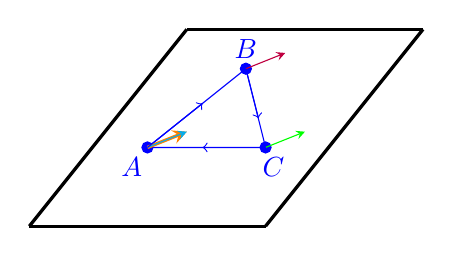
\begin{tikzpicture}
 					\draw [very thick] (-1,-2) -- (1,0.5);
 					\draw [very thick] (2,-2) -- (4,0.5);
 					\draw [very thick] (-1,-2) -- (2,-2);
 					\draw [very thick] (1,0.5) -- (4,0.5);
 					
 					\filldraw [blue] (0.5, -1) circle (2pt) node [left=2mm, below] {$A$}
 						 (2, -1) circle (2pt) node [right=1mm, below] {$C$}
 						 (1.75, 0) circle (2pt) node [above] {$B$};
 					\draw [blue] (0.5, -1) -- (2,-1) -- (1.75, 0) -- (0.5, -1);
 					
 					\draw [->, very thick, orange, >=stealth] (0.5, -1) -- (1, -0.8) ; 
 					\draw [->, cyan, >=stealth] (0.5, -1) -- (1, -0.8) ;
 					\draw [->, purple, >=stealth] (1.75, 0) -- (2.25, 0.2) ; 
 					\draw [->, green, >=stealth] (2, -1) -- (2.5, -0.8) ; 
 					
 					\draw [->, blue] (0.5, -1) -- (1.2, -0.44);
 					\draw [->, blue] (1.75, 0) -- (1.91, -0.63);
 					\draw [->, blue] (2, -1) -- (1.2, -1);
 					
 						
 				\end{tikzpicture}
 				\vspace{0.5cm}
 				\caption{Triangle over a flat manifold. We consider a vector $v^\mu$ on vertex $A$ and transport it to vertex $B$, then to vertex $C$, and then finally to vertex $A$ again. In this cycle, the vector will not rotate while translating over the manifold.}
 			\end{minipage}
 			\hfill
 			\begin{minipage}{0.46\textwidth}
 				\center
 				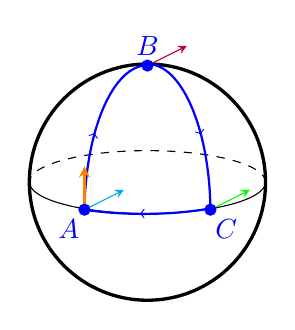
\begin{tikzpicture}
 					\draw [very thick] (0,0) circle (1.5cm);
 					\draw [dashed] (1.5,0) arc (0:180:1.5 and 0.4);
 					\draw (1.5,0) arc (0:180:1.5 and -0.4);
 					
 					\draw [thick, blue] (0.8, -0.35) arc (1.5:90:0.8 and 1.9);
 					\draw [thick, blue] (-0.8, -0.35) arc (178:90:0.8 and 1.9);
 					\draw [thick, blue] (-0.8, -0.35) arc (120:58:1.5 and -0.4);
 					
 					\draw [->, thick, orange, >=stealth] (-0.8, -0.35) -- (-0.8, 0.2) ; 
 					\draw [->, purple, >=stealth] (0, 1.48) -- (0.5, 1.73) ; 
 					\draw [->, green, >=stealth] (0.8, -0.35) -- (1.3, -0.1) ; 
 					\draw [->, cyan, >=stealth] (-0.8, -0.35) -- (-0.3, -0.1) ; 
 					
 					\filldraw [blue] (0.8,-0.35) circle (2pt) node [right=2mm, below] {$C$}
 					(0,1.48) circle (2pt)  node [above] {$B$}
 					(-0.8, -0.35) circle (2pt)  node [left=2mm, below] {$A$};
 					
 					\draw [->, blue] (-0.68, 0.6) -- (-0.67, 0.63);
 					\draw [->, blue] (0.67, 0.63) -- (0.68, 0.6);
 					\draw [->, blue] (0.1, -0.4) -- (-0.1, -0.4);
 					
 					
 				\end{tikzpicture}
 				\caption{We consider a vector $v^\mu$ on vertex $A$ and transport it to vertex $B$, then to vertex $C$, and then finally to vertex $A$ again. In this cycle, the vector will rotate accordingly as it translates over the manifold, so when it returns to point $A$ it will not point in the same direction as in the initial position.}
 			\end{minipage}
 		\end{figure}
 	
 	\noindent
 		The notion above captures the fact that vectors fail to conserve their direction when they are translated over a curved manifold. In order to make this precise, we need to understand how vectors can change when they are transported around cycles as the ones in Fig. 11 and Fig. 12.
 		
 		\begin{thm}
 			A vector $w^\mu$ is transported in parallel along a worldline $x^\mu (\lambda)$ if 
 			\begin{equation}
 				\label{eq:ParallellyTransported}
 				\boxed{v^\mu \Del_\mu w^\nu = 0}
 			\end{equation}
 			Where $v^\mu = \dot{x}^\mu = \frac{dx^\mu}{d\lambda}$ 
 		\end{thm}
 		\begin{exmp}
 			A geodesic has the property that the tangent vector of the curve is parallelly trasported to itself as you move along the curve.
 			$$ v^\mu \Del_\mu v^\rho = f(\lambda)v^\rho$$
 			
 			\begin{figure}[h]
 				\begin{minipage}{0.46\textwidth}
 					\centering
 					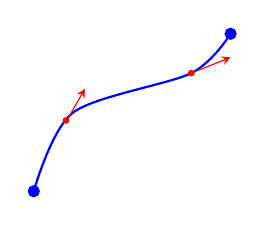
\begin{tikzpicture}
 							\draw [thick, blue] plot [smooth] coordinates{(-1,-1) (-0.5, 0) (1, 0.5) (1.5, 1)};
 							\filldraw [blue] (-1,-1) circle (2pt)
 							(1.5,1) circle (2pt);
 							
 							\filldraw [red] (-0.59,-0.1) circle (1pt)
 							(1,0.5) circle (1pt);
 							\draw [->, >=stealth, red] (-0.58, -0.1) -- (-0.35, 0.3);
 							\draw [->, >=stealth, red] (1, 0.5) -- (1.5, 0.7);
 					\end{tikzpicture}
 					\vspace{0.45cm}
 					\caption{Not a geodesic as the tangent vector is not parallel to the curve for all points on the curve.}
 				\end{minipage}
 				\hfill
 				\begin{minipage}{0.46\textwidth}
 					\centering
 					\begin{tikzpicture}
 						\draw [thick, blue] plot [smooth] coordinates{(-1,-1) (1.5, 1.5)};
 						\filldraw [blue] (-1,-1) circle (2pt)
 						(1.5,1.5) circle (2pt);
 						
 						\filldraw [red] (-0.3,-0.3) circle (1pt)
 						(0.5,0.5) circle (1pt);
 						\draw [->, >=stealth, red] (-0.3, -0.3) -- (0, 0);
 						\draw [->, >=stealth, red] (0.5, 0.5) -- (0.8, 0.8);
 					\end{tikzpicture}
 					\caption{A geodesic as the tangent vector is parallel to the curve for all points on the curve.}
 				\end{minipage}
 			\end{figure}
 		\end{exmp}
 		So how does a vector change as we parallel transport it around some small cycle in spacetime? Let us start by defining a parallelogram. We define each edge of the parallelogram as a directional vector from one vertex to another.
 		\begin{figure}[h]
 			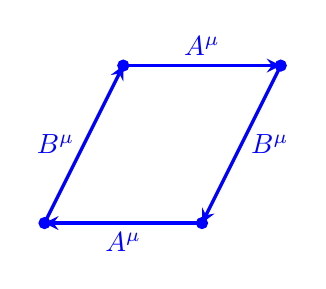
\begin{tikzpicture}
 				\filldraw [blue]
 					(0,0) circle (2pt) 
 					(2,0) circle (2pt)
 					(1,2) circle (2pt)
 					(3,2) circle (2pt);
 				\draw [->, very thick, blue, >=stealth] (0,0) -- (1,2); 
 				\draw [blue] (0.5, 1) node [left] {$B^\mu$};
 				\draw [->, very thick, blue, >=stealth] (1,2) -- (3,2); 
 				\draw [blue] (2, 2) node [above] {$A^\mu$};
 				\draw [->, very thick, blue, >=stealth] (3,2) -- (2,0); 
 				\draw [blue] (2.5, 1) node [right] {$B^\mu$};
 				\draw [->, very thick, blue, >=stealth] (2,0) -- (0,0); 
 				\draw [blue] (1, 0) node [below] {$A^\mu$};
 			\end{tikzpicture}
 		\end{figure}
 	
 		Given a displacement given by $x^\mu \to x^\mu + B^\mu$, we yield a change in vectors given by
 		\begin{equation}
 			\label{eq:VectorChange}
 			v^\mu \to v^\mu + B^\alpha \Del_\alpha v^\mu + \dots
 		\end{equation}
 		So if we transport the vector around the cycle given by the parallelogram, we have a variation
 		\begin{equation}
 			\label{eq:VectorVariation}
 			\delta v^\rho = A^\mu B^\nu \left[ \Del_\mu, \Del_\nu \right] v^\rho 
 		\end{equation}
 		Furthermore, if $x^\mu + B^\mu \to x^\mu + B^\mu + A^\mu$, then
 		\begin{equation}
 			\label{eq:VectorChange2}
 			v^\mu  B^\alpha \to v^\mu + B^\alpha \Del_\alpha v^\mu + A^\beta \Del_\beta \left( v^\mu + B^\alpha \Del_\alpha v^\mu \right) + \dots 
 		\end{equation}
 		So
 		\begin{equation}
 			\label{eq:VectorVariation2}
 			\delta v^\rho = A^\mu B^\nu \left[ \Del_\mu, \Del_\nu \right] v^\rho  = A^\mu A^\nu \left( \Del_\mu 
 			\Del_\nu - \Del_\nu \Del_\mu \right)
 		\end{equation}
 		
 		This is a characterization of the local curvature at some point in spacetime. We are considering initial points and subsequent infinitesimal displacements from said points.
 		\begin{defn}
 			The \textbf{Riemann curvature tensor} $R^{\rho}_{\sigma\mu\nu}$ of some vector $v^\rho$ in terms of the commutator of covariant derivatives $\left[\Del_\mu, \Del_\nu \right]$ and arbitrary infinitesimal displacement vectors $A^\mu$ and $B^\nu$ is a (1,3)-tensor that defines the change in $v^\rho$ over displacements $A^\mu$ and $B^\mu$ given the curvature of a manifold as given by $\left[\Del_\mu, \Del_\nu \right]$, such that
 			\begin{equation}
 				\label{eq:RiemannTensor}
 				\boxed{\delta v^\rho = R^\rho_{\sigma \mu \nu} A^\mu B^\nu v^\rho}
 			\end{equation}
 			The Riemann tensor is antisymmetric in the last two indices $\mu \leftrightarrow \nu$. 
 		\end{defn}
 		This tensor tells us about curvature in different directions over some manifold. However, we can give a much more explicit definition of the tensor itself by computing it. First, we have the commutator of two covariant derivatives acting on a vector such that:
 		\begin{align*}
 			\left[\Del_\mu, \Del_\nu \right] v^\rho &= \Del_\mu \left( \Del_\nu v^\rho\right) - \Del_\nu \left( \Del_\mu v^\rho \right) \\
 			&= \partial_\mu \left( \Del_\nu v^\rho \right) - \Gamma^\lambda_{\mu\nu} \Del_\lambda v^\rho + \Gamma_{\mu\sigma}^\rho \Del_\nu v^\sigma - \partial_\nu \left( \Del_\mu v^\rho \right) + \Gamma^\lambda_{\nu\mu} \Del_\lambda v^\rho - \Gamma_{\nu\sigma}^\rho \Del_\mu v^\sigma \\
 			&= \partial_\mu \left( \partial_\nu v^\rho\right) + \partial_\mu \left(\Gamma_{\nu\sigma}^\rho v^\sigma \right) + \Gamma_{\mu\sigma}^\rho \partial_\nu v^\sigma + \Gamma_{\mu\sigma}^\rho \Gamma_{\nu\lambda}^\sigma v^\lambda  \\
 			&\quad\quad\quad\quad\quad\quad\quad\quad\quad\quad- \partial_\nu \left( \partial_\mu v^\rho\right) - \partial_\nu \left(\Gamma_{\mu\sigma}^\rho v^\sigma \right) - \Gamma_{\nu\sigma}^\rho \partial_\mu v^\sigma - \Gamma_{\nu\sigma}^\rho \Gamma_{\mu\lambda}^\sigma v^\lambda \\
 			&= v^\sigma \left( \partial_\mu \Gamma_{\nu\sigma}^\rho + \Gamma_{\mu\lambda}^\rho \Gamma_{\nu\sigma}^\lambda - \partial_\nu \Gamma_{\mu\sigma}^\rho - \Gamma_{\nu\lambda}^\rho \Gamma_{\mu\sigma}^\lambda \right)\\
 			&= R^{\rho}_{\sigma\mu\nu}v^\sigma 
 		\end{align*}
 		And so
 		\begin{equation}
 			\label{eq:CurvatureTensor}
 			\boxed{R^\rho_{\sigma\mu\nu} =  \partial_\mu \Gamma_{\nu\sigma}^\rho - \partial_\nu \Gamma_{\mu\sigma}^\rho + \Gamma_{\mu\lambda}^\rho \Gamma_{\nu\sigma}^\lambda - \Gamma_{\nu\lambda}^\rho \Gamma_{\mu\sigma}^\lambda}
 		\end{equation}
 		We now define a few properties of the Riemann tensor:
 		\begin{enumerate}[$\quad\quad$(1)]
 			\item \textbf{The Riemann tensor is a tensor}
 				\subitem 
 				The Riemann tensor $R^\rho_{\sigma\mu\nu}$ as given in Definition 3.1 is a (1,3)-tensor despite our knowledge that the Christoffel symbol is not a tensor. We can show this by recalling that the definition is given in terms of covariant derivatives, and as they give a tensor to tensor transformation, they themselves must be a tensor. This means that the Riemann tensor is a covariant notion of curvature, that is, it is independent of choice of coordinates.
 				\begin{thm}
 					If we find that $R^\rho_{\sigma\mu\nu} = 0$, then we say that spacetime is flat.
 				\end{thm}
 			\item \textbf{Constant metric and flatness}
 				\subitem
 				If there exists a coordinate system where the metric is constant, then in that metric the Christoffel symbol clearly vanishes and hence so does the Riemann tensor. On the other hand, we consider as a fact that a flat spacetime implies that there is a coordinate system where the metric is constant.
 				\begin{thm}
 					Spacetime is said to be flat if and only if there exists a coordinate system where the metric $g_{\mu\nu}$ is constant such that $\Gamma^\rho_{\mu\nu} = 0$.
 				\end{thm}
 			\item \textbf{Symmetries}
 				\subitem 
 				We use the inverse of the metric as usual to lower the index of a Riemann tensor
 				\begin{equation}
 					\label{eq:RiemannLower}
 					R_{\rho\sigma\mu\nu} = g^{\rho\alpha} R^\alpha_{\sigma\mu\nu}
 				\end{equation}
 				\begin{thm}
 					Lowering indices for a Riemann tensor leads to the symmetries
 					\begin{equation}
 						\label{eq:RiemannSymmetry}
 						\boxed{R_{\rho\sigma\mu\nu} = -R_{\rho\sigma\nu\mu}}
 					\end{equation}
 					\begin{equation}
 						\label{eq:RiemannSymmetry2}
 						\boxed{R_{\rho\sigma\mu\nu} = -R_{\sigma\rho\mu\nu}}
 					\end{equation}
 					\begin{equation}
 						\label{eq:RiemannSymmetry3}
 						\boxed{R_{\rho\sigma\mu\nu} = -R_{\mu\nu\rho\sigma}}
 					\end{equation}
 					And anti-symmetrization over all the indices gives
 					\begin{equation}
 						\label{eq:RiemannAntiSymmetry}
 						\boxed{R_{\left[ \rho\sigma\mu\nu \right]} = 0}
 					\end{equation}
 				\end{thm}
 		\end{enumerate}
 		\begin{defn}
			The \textbf{Ricci curvature tensor} $R_{\mu\nu}$ is a symmetric (0,2)-tensor arising from a contraction of the contravariant and the second covariant index of the Riemann Tensor $R^{\rho}_{\mu\sigma\nu}$ such that
			\begin{equation}
				\label{eq:RicciTensor}
				\boxed{R_{\mu\nu} = R^{\rho}_{\mu\rho\nu}}
			\end{equation}
		\end{defn}
		From the definition, we can see that indeed it is a symmetric tensor
		\begin{equation}
			R_{\mu\nu} = R_{\nu\mu}
		\end{equation}
	 	\begin{defn}
	 		The \textbf{scalar curvature tensor} is a (0,0)-tensor given by contracting the indices of the Ricci tensor $R_{\mu\nu}$ with the inverse metric $g^{\mu\nu}$ such that
	 		\begin{equation}
	 			\label{eq:ScalarCurvature}
	 			\boxed{R = R_{\mu\nu} g^{\mu\nu} }
	 		\end{equation}
	 	\end{defn}
 		We are developing a brief but comprehensive theory of differential geometry to better introduce general relativity, as this is the language it is defined in. In general relativity, the effect of gravity is described by the curvature of spacetime, which implies that the equation of motion for spacetime is going to be an equation involving the Riemann tensor. So what equations of gravitation can we write? One possibility to describe the curvature of spacetime, we write $R^{\rho}_{\mu\nu\sigma} = 0$. However, we know this is Minkowski spacetime so there is no curvature in the metric, so this is far too simple to study General Relativity. The next simplest equation would be when the Ricci tensor vanishes, which is known as \textbf{Einstein's equation in the absence of matter.}
 		\begin{equation}
 			\label{eq:EinsteinEquation0}
 			\boxed{R_{\mu\nu} = 0}
 		\end{equation}
 		\begin{exe}
 			Consider the manifold $\R^2$ with two coordinate systems $x^\mu = (x,y)$ and $x^{\mu'} = (r,\theta)$ such that
 			$$ ds^2 = dx^2 + dy^2 = dr^2 + r^2 d\theta^2$$
 			Here, we have $\Gamma_{\theta\theta}^r = -r$ and $\Gamma_{r\theta}^\theta = \frac{1}{r}$. Compute the Riemann tensor in both coordinate systems.
 		\end{exe}
 		We now recall that from a metric $g_{\mu\nu}$ we obtain the \hyperref[eq:ChristoffelSymbol]{Christoffel Symbol}, which is not a tensor and it captures the deviation of a particle from being in a straight line. It achieves this capture using the effect of fictitious forces in an accelerating coordinate system as well as the effect of some curvature in the geometry of the metric. In order to get this notion of curvature, we observed how vectors transform over cycles in spacetime using the \hyperref[eq:RiemannTensor]{Riemann Tensor}, which is defined by a linear combination of the first derivatives of the Christoffel symbol and the squares of the Christoffel symbol. In other words, the Riemann tensor captures the extent to which spacetime is not flat. So it is impossible to find a coordinate system where the metric is constant.
 		
 		The \hyperref[defn:StrongEquivalence]{Equivalence Principle} states that for any point $x_0^\mu$ in spacetime given coordinates $x^\mu$, we can find a new coordinate system $x^{\mu'}$ which has the property that at this point $x_0^\mu = x^{\mu'} = 0$ we have:
 		\begin{equation}
 			\label{eq:FlatMetric2}
 			g_{\mu'\nu'} = \eta_{\mu' \nu'}
 		\end{equation}
 		For this, we consider a metric $g_{\mu\nu}$ in some coordinates $x^\mu$. Now define a new coordinate system $x^{\mu'}$ such that the metric 
 		becomes
 		\begin{equation}
 			\label{eq:MetricTransform}
 			\boxed{g_{\mu'\nu'} = \frac{\partial x^\mu}{\partial x^{\mu'}} \frac{\partial x^\nu}{\partial x^{\nu'}} g_{\mu\nu}}
 		\end{equation} 
 		We now Taylor expands both sides in powers of $x^{\mu'}$ around the point $x^{\mu'} = 0$. At this point, the metric $g_{\mu\nu}$ has 10 degrees of freedom and the Jacobian $\frac{\partial x^{\mu}}{\partial x^{\mu'}}$ is a $4\times 4$ matrix with 16 degrees of freedom. This implies that we can choose a Jacobian such that we yield equation (\ref{eq:FlatMetric2}). So we adjust the free parameters in the Jacobian that we've used when referring to the Equivalence Principle.
 		
 		If we now consider the neighbourhood around $x^{\mu'} = 0$, we now expand the Jacobian in terms in order of powers of $x^{\mu'}$.
 		\begin{align*}
 			\frac{\partial x^\mu}{\partial x^{\mu'}} &= \left. \frac{\partial x^\mu}{\partial x^{\mu'}} \right|_{x^{\mu'} = 0} + \left. \frac{\partial^2 x^\mu}{\partial x^{\mu'} \partial x^{\nu'} } \right|_{x^{\mu'} = 0} x^{\mu'} + \left. \frac{\partial^3 x^{\mu}}{\partial x^{\mu'} \partial x^{\nu'} \partial x^{\sigma'} }\right|_{x^{\mu'} = 0} \left( x^{\mu'} \right)^2 + \cdots 
 		\end{align*}
 		On the expansion, the first term has $4\times 4 = 16$ degrees of freedom as it is the Jacobian as usual, the second term has $4 \times 10 = 40$ degrees of freedom as we have 4 choices for the coordinates and 10 degrees of freedom in a symmetric (2,0)-tensor, and the third term has $4 \times 20 = 80$ degrees of freedom given the 4 choices of coordinates and the 20 degrees of freedom in a symmetric (3,0)-tensor. We remember that we are attempting to compare these degrees of freedom to the number of degrees of freedom in $g_{\mu'\nu'}$ expanded around $x^{\mu'} = 0$.
 		$$ g_{\mu'\nu'} = \left. g_{\mu'\nu'} \right|_{x^{\mu'} = 0} + \left. \partial_{\mu'} g_{\mu'\nu'} x^{\mu'} \right|_{x^{\mu'} = 0}+ \left. \partial_{\mu'} \partial_{\nu'} g_{\mu'\nu'} \right|_{x^{\mu'} = 0} \left( x^{\mu'}\right)^2 + \cdots$$
 		On this expansion we know the metric will have 10 degrees of freedom. The derivative of the metric will be over 4 coordinates, so it will be $4 \times 10 = 40$ degrees of freedom on the second term. The third term will be the number of degrees of freedom in the metric squared, so it will have $10^2 = 100$ degrees of freedom. 
 		
 		Let us do this explicitly by expanding at $\mathcal{O}\Big(\big(x^{\mu'} \big)^0\Big)$. As we saw for equation (\ref{eq:FlatMetric2}), the 16 degrees of freedom in the Jacobian allow us to have the metric equal to a Minkowski metric. For $\mathcal{O}\Big(\big(x^{\mu'} \big)^1\Big)$ we have the same number of degrees of freedom which allows us to say $\partial g_{\mu'\nu'} = 0$. At order $\mathcal{O}\Big(\big(x^{\mu'} \big)^2\Big)$ we have a 20 degree of freedom difference, so we have 20 degrees of freedom in the second derivative of the metric that cannot be removed by some choice of coordinates.
 		
 		To summarize this, we can always choose coordinates where the metric is the flat metric and the first derivative of the metric vanishes at any given point, which in the above example we chose to be the origin $x^{\mu'}=0$
 		$$ g_{\mu' \nu'} = \eta_{\nu'\mu'} \quad\quad \text{AND} \quad \quad \partial_{\rho'} g_{\mu' \nu} = 0$$
 		\begin{defn}
 			\label{defn:RNC}
 			The coordinates $x^{\mu'}$ that allow for a flat metric $g_{\mu' \nu'} = \eta_{\nu'\mu'}$ and a zero first derivative at any point $\partial_{\rho'} g_{\mu' \nu} = 0$ are denoted \textbf{Riemann Normal Coordinates} or \textbf{Locally Inertial Coordinates} or \textbf{Freely Falling Coordinates}.
 		\end{defn}
 		Recalling Einstein's elevator accelerating downwards at $9.8$ m s$^{-2}$, one would experience a net zero force and would not move on the reference frame of the elevator, considering the elevator is falling towards the Earth. This technique is how airplanes emulate zero-gravity. Thus, we can also extrapolate this to General Relativity where $\Gamma_{\mu'\nu'}^{\rho'} = 0$ for some given point. So now it is natural to wonder what the Riemann tensor would be in Riemann Normal Coordinates. We first lower the Riemann tensor index and define it at the point $x^{\mu'} = 0$.
 		\begin{align*}
 			R_{\rho'\sigma'\mu'\nu'} &= g_{\rho'\alpha'} R^{\alpha'}_{\sigma'\mu'\nu'} \\
 			&= g_{\rho'\alpha'} \left( \partial_{\mu'} \Gamma_{\sigma'\nu'}^{\alpha'} - \partial_{\nu'} \Gamma_{\sigma'\nu'}^{\alpha'} \right) \\
 			&=  g_{\rho'\alpha'} \left( \partial_{\mu'} \left( \frac12 g^{\alpha'\beta'} \left( g_{\sigma'\beta';\nu'} + g_{\nu'\beta';\sigma'} - g_{\sigma'\nu';\beta'}\right)\right) - \partial_{\nu'} \left( \frac12 g^{\alpha'\beta'} \left( g_{\sigma'\beta';\mu'} + g_{\mu'\beta';\sigma'} - g_{\sigma'\mu';\beta'}\right)\right) \right) \\
 			&= \frac12 \left( \partial_{\mu'} \left( \partial_{\nu'} g_{\sigma'\rho'} + \partial_{\sigma'} g_{\nu'\rho'} - \partial_\rho g_{\sigma'\nu'}\right) - \partial_{\nu'} \left( \partial_{\mu'} g_{\sigma' \rho'} + \partial_{\sigma'} g_{\mu'\rho'} - \partial_{\rho'} g_{\sigma'\mu'}\right)\right) \\
 			&= \frac12 \left( \partial_{\mu'} \partial_{\sigma'} g_{\nu'\rho'} - \partial_{\mu'} \partial_{\rho'} g_{\sigma'\nu'} - \partial_{\nu'} \partial_{\sigma'} g_{\rho'\mu'} + \partial_{\nu'} \partial_{\rho'} g_{\sigma'\mu'} \right)
 		\end{align*}
 		This implies symmetries from the properties of the Riemann tensor
 		\begin{align*}
 			R_{\rho'\sigma'\mu'\nu'} &= -R_{\rho'\sigma'\nu'\mu'} \\
 			 &= - R_{\sigma'\rho'\mu'\nu'} \\
 			 &= R_{\mu'\nu'\rho'\sigma'}
 		\end{align*}
 		And the anti-symmetry:
 		$$ R_{\left[ \rho' \sigma' \mu'\nu' \right]} = R_{\rho' \left[\sigma'\mu'\nu'\right]}=0$$
 		
 		So we made a clever choice of coordinates which allowed us to evaluate the Riemann tensor at the point $x^{\mu'} = 0$. So given these symmetry conditions, we find the degrees of freedom in the Riemann tensor. Equations (\ref{eq:RiemannSymmetry}) and (\ref{eq:RiemannSymmetry2}) imply that the first and second pairs of indices in the Riemann tensor each act like a $4 \times 4$ anti-symmetric matrix, meaning we have $\frac{4\times3}{2} = 6$ degrees of freedom. Recall that for $D$-dimensions, a square matrix has $D^2$ degrees of freedom, a symmetric matrix has $\frac{(D+1)D}{2}$ degrees of freedom, and an anti-symmetric matrix has $\frac{D(D-1)}{2}$ degrees of freedom. Equation (\ref{eq:RiemannSymmetry3}) implies that the Riemann tensor itself behaves like a symmetric $6 \times 6$ matrix, so we have $\frac{6\times7}{2}=21$ degrees of freedom. Finally, equation (\ref{eq:RiemannAntiSymmetry}) removes the number of degrees of freedom in a 4-index anti-symmetric tensor, so it removes 1 degree of freedom. In conclusion, the number of degrees of freedom in a Riemann tensor has $21-1=20$ degrees of freedom.
 		\begin{rem}
 			The Riemann tensor $R^\rho_{\sigma\mu\nu}$ is a packaging of the 20 independent degrees of freedom in the second derivative of the metric $\partial^2 g$ into a tensor.
 		\end{rem}
 		\begin{defn}
 			The \textbf{Binachi Identity} is a property of the first derivative of a Riemann tensor with respect to $\lambda$ such that
 			\begin{equation}
 				\label{eq:BinachiIdentity}
 				\boxed{\Del_{\left[\lambda \right.} R_{\left. \rho \sigma \right] \mu\nu}}
 			\end{equation}
 		\end{defn}
 		So we defined the Ricci tensor as the trace of the Riemann tensor (\ref{eq:RicciTensor}), and we defined the Scalar curvature as the trace of the Ricci scalar (\ref{eq:ScalarCurvature}). Hence, by the Binachi identity we can show that
 		\begin{equation}
 			\label{eq:BinachiIdentityApplied}
 			\boxed{\Del^\mu R_{\mu\nu} = \frac12 \Del_\nu R}
 		\end{equation}
 		\begin{defn}
 			We define the \textbf{Einstein Tensor} as
 			\begin{equation}
 				\label{eq:EinsteinTensor}
 				\boxed{G_{\mu\nu} = R_{\mu\nu} - \frac12 g_{\mu\nu} R}
 			\end{equation}
 		\end{defn}
 		The Binachi identity and the Einstein tensor yield
 		\begin{equation}
 			\label{eq:EinsteinTensorBinachi}
 			\boxed{\Del^\mu G_{\mu\nu} = 0}
 		\end{equation}
 		
 	\begin{exe}
 		Consider the wavefunction $\Psi (x) \to e^{i \Lambda} \Psi (x)$ of a particle where we transform the wavefunction by multiplication of some phase $e^{i\Lambda}$. Show that to develop a theory of physics where that phase is allowed to depend where you are in space we would require another degree of freedom, which is the electromagnetic field. The phase transformation in Quantum Mechanics is promoted to a local symmetry which is identified with the Gauge transformation in electromagnetism. (\textit{Hint: Consider the Aharonov-Bohm effect.})
 	\end{exe}
 	\begin{exe}
 		Consider the wavefunctions $\Psi_i (x) \to U_i^j \Psi_i (x)$ of a system of $i$ particles where we transform the wavefunction by multiplication of some Unitary $3 \times 3$ matrix $U^j_i$. Show that to develop a theory of physics where that phase is allowed to be independent of position in spacetime, we would need to introduce $i$ degrees of freedom. For the case where $i=3$, we call these degrees of freedom \textbf{gluons} and the particles \textbf{quarks}, albeit in 2015 \href{https://journals.aps.org/prl/abstract/10.1103/PhysRevLett.115.072001}{CERN} found evidence of quarks in groups of 5, called \textbf{pentaquark particles}, and before that quarks in groups of four were also found in \href{https://journals.aps.org/prl/abstract/10.1103/PhysRevLett.110.252001}{Beijing} and \href{https://journals.aps.org/prl/abstract/10.1103/PhysRevLett.110.252002}{Tsukuba}, denoted \textbf{tetraquark particles}.
 	\end{exe}
 	
 	\pagebreak
 	\section{General Theory of Relativity}
 	\subsection{Gravitation}
 		How can we begin to formulate the laws of physics in the geometry of curved spacetime? More precisely, let us imagine that we know the laws of physics in flat space, ie. Special Relativity. We now need to find how to translate these well-known laws of physics into laws of physics that are valid for curved spacetime. We begin by assuming we know some laws of physics, like the laws of electromagnetism or mechanics. From the \hyperref[defn:StrongEquivalence]{Equivalence Principle} we know that the laws of physics can be studied in a considerably small region such that the laws of physics in this small frame of reference are equivalent to those of Special Relativity, albeit possibly in some inertial coordinate system. So near any particular point $x^\mu_0$ in spacetime, there exists some inertial coordinate system $x^{\hat\mu}$(which we previously defined as \hyperref[defn:RNC]{Riemann Normal Coordinates}) such that the metric is approximately flat.
 		$$ g_{\hat\mu\hat\nu} = \eta_{\hat\mu\hat\nu} + \mathcal{O}\left( \partial g \left. x \right|_{x^{\mu}_0}  \right)$$
 		Where $\mathcal{O}\left( \partial g \left. x\right|_{x^\mu_0} \right)$ denotes the vanishing first and higher order derivatives of the metric $g_{\mu\nu}$ at the point $x^\mu_0$ such that the only non-vanishing term on the RHS is $\eta_{\hat\mu\hat\nu}$. Also, do not feel confused by the use of $x^{\hat\mu}$ rather than $x^{\mu'}$ as done at the end of chapter 2. Both notations define some inertial coordinate system over the same manifold, so the choice of which one to use for the examples is completely arbitrary, but must remain consistent once it is used to define an inertial coordinate system.
 		
 		Let us consider a set of laws of physics in Special Relativity such that we define them over some locally Minkowski spacetime manifold $\R^{3,1}$ around some particular point $x^\mu_0$, but which curves in the neighbourhood around $x^{\mu}_0$. Then, we must proceed to define every law of physics in tensorial form, such that every equation of motion is written with tensors but in an inertial coordinate system $x^{\hat\mu}$ adapted at the point $x^\mu_0$. If everything is done correctly and follows the mathematics established in chapter 2, then we find that the tensor equation we get for every law of physics represents said law of physics in curved spacetime. This effectively yields a transition from laws of physics in flat spacetime to the same laws of physics in curved spacetime. 
 		
 		\begin{defn}
 			The \textbf{Principle of Minimal Coupling} allows any set of laws of physics well-defined on flat spacetime to be covariantly transformed into tensor equations via the transformation
 			\vspace{1.5cm}
 			\begin{equation}
 				\label{eq:PrincipleOfMinimalCoupling}
 				\boxed{ \text{PMC} \equiv \begin{cases}
 						\eta_{\mu\nu} \to g_{\mu\nu} \\
 						\frac{\partial}{\partial x^\mu} \to \Del_\mu
 				\end{cases}}
 			\end{equation}
 		\end{defn}
 	
 		\pagebreak
 		
 		\begin{exmp}
 			\textbf{Newton's Laws of Motion}\\
 			According to Newton's laws of motion, any object that is not acted on by any external force will have constant velocity. Moreover, a particle in Special Relativity that does not interact with any external forces will also have constant velocity. We define an affine parameter $\lambda$ to denote a worldline $x^\mu (\lambda)$ for some particle with constant velocity in special relativity such that $\lambda$ is proportional to the proper time of the particle. Then, allowing differentiation with respect to $\lambda$, we have:
 			\begin{equation}
 				\label{eq:Newton1}
 				\frac{d^2}{d\lambda^2} x^\mu = \ddot{x}^\mu = 0
 			\end{equation}
 			This is not a tensorial equation. To see this, define $v^\nu \partial_\nu v^\mu = 0$ where $v^\mu = \dot{x}^\mu$. By the chain rule, the particle with constant velocity in Special Relativity will include a partial derivative and thus cannot be a tensorial equation. We need to covariantize via the Principle of Minimal Coupling to turn this into a tensorial equation, which becomes the \hyperref[eq:GeodesicEquation]{Geodesic Equation}
 			\begin{equation}
 				\label{eq:Newton2}
 				v^\nu \Del_\nu v^\mu = \ddot{x}^\mu + \Gamma_{\nu\rho}^\mu \,\dot{x}^\nu \dot{x}^\rho = 0
 			\end{equation}
 			Moreover, free-falling particles will follow geodesics over curved spacetime. This results in gravity not being a force, but rather a feature of the curvature of spacetime. Therefore, the geodesic equation will have to capture the effect of gravity on the motion of the particle. This constricts the notion of no external forces to exclude gravitation, as it is therefore not a force. So we can say that the effect of gravity on the motion of particles is that they should travel on geodesics, as long as they are not acted on by our other forces aside from gravity.
 		\end{exmp}
 		So how does geodesic motion through curved space reproduce properties of gravity that we already know, such as Kepler's laws and Newtonian gravitation? Let us consider a particle in some Cartesian coordinates $x^\mu$ over some Manifold $M$ that is locally flat. This implies that the gravitational field is weak. Second, we consider that the particle is moving relatively slowly, such that its speed at any point has the property $v \ll c$, thereby making relativistic effects negligible. In a more generalized sense:
 		$$ x^\mu = (x^0, x^1, x^2, x^3) = (x^0, x^i)$$
 		$$ \therefore \dot{x}^0 \approx 1 \quad\quad \text{AND} \quad\quad \dot{x}^i \ll c$$
 		Where we have that $\dot{x}^\mu = \frac{d}{d\lambda} x^\mu$ and $\lambda \approx t$. As in the case of the Newtonian example, $\lambda$ represents the proper time $t \approx \tau$ for the particle. Thus, we would get a geodesic equation for the particle as in equation (\ref{eq:Newton2}). From the geodesic equation, we would like to find the acceleration of the particle meaning we only work with the spatial coordinate indices $i$. This yields:
 		\begin{equation}
 			\label{eq:ParticleAcceleration}
 			\boxed{\ddot{x}^{i} = -\Gamma_{\nu\rho}^i \dot{x}^\nu \dot{x}^\rho \approx - \Gamma_{00}^i \left( \dot{x}^0 \right)^2 \approx - \Gamma_{00}^i}
 		\end{equation}
 		So the acceleration of a particle relates to the first derivatives of the metric through $-\Gamma_{00}^i$. We now wish to compare this result to Newton's gravitation law that describes the motion of a particle in a gravitational field. Recall that Newton's gravitation law implies that
 		\begin{equation}
 			\label{eq:NewtonGravitation}
 			\ddot{\vec{x}} = - \vec{\Del} \Phi
 		\end{equation}
 		Where we have that $\vec{\Del} \Phi$ represents the force of the gravitational potential function $\Phi$. We can thus make an analogy that $\Phi \approx g_{\mu\nu}$ and therefore $\vec{\Del}\Phi \approx \Gamma_{ij}^k$. Let us now imagine that $g_{\mu\nu} \approx \eta_{\nu\mu}$ such that there exists a Cartesian coordinate system where
 		\begin{equation}
 			\label{eq:Deviation}
 			g_{\mu\nu} = \eta_{\mu\nu} + h_{\mu\nu} = \eta_{\mu\nu} + \mathcal{O}\left(h\right)
 		\end{equation}
 		Where $h_{\mu\nu}$ represents the small deviation from being flat. This means that 
 		\begin{equation}
 			\label{eq:InverseDeviation}
 			g^{\mu\nu} = \eta^{\mu\nu} + h^{\mu\nu} = \eta^{\mu\nu} + \mathcal{O}\left(h\right)
 		\end{equation}
 		The Christoffel symbol of this nearly flat metric will hence be
 		\begin{equation}
 			\label{eq:FlatChristoffels}
 			\Gamma_{\nu\rho}^{\mu} = \frac12 \eta^{\mu\nu} \left( h_{\sigma\nu;\rho} + h_{\sigma\rho;\nu} - h_{\nu\rho;\sigma} \right) + \bigO \left( h^2 \right)
 		\end{equation}
 		Now let us imagine that the metric is static with respect to the Cartesian coordinates, and also consider that the metric is independent of time such that $h_{\mu\nu}$ is also independent of time. Thus, we can use equation (\ref{eq:ParticleAcceleration}) and compute $\Gamma_{00}^i$
 		\begin{equation}
 			\label{eq:ChristoffelAcceleration}
 			\Gamma_{00}^i = - \frac12 h_{00;i}
 		\end{equation}
 		So the geodesic equation for a particle moving relatively slowly through an approximately flat spacetime where we can consider time to be independent of space as:
 		$$ 
 			\ddot{x}^i = -\frac12 h_{00;i} \implies \ddot\vec{x} = -\vec\Del \left( \frac12 h_{00;i} \right) 
 		$$
 		Notice that because spacetime is flat, we are allowed to switch between upper and lower indices so the above equation still holds. This means that \textit{the geodesic equation is the force law of Newtonian gravity for metrics which are static and nearly flat, and for particles that are moving slowly}. For this to hold, we must set
 		\begin{equation}
 			\label{eq:GravityForce}
 			h_{00}^i = -2 \Phi
 		\end{equation}
 		In other words, Newtonian gravity might have been considered as the effects of gravitational fields on objects in spacetime. But more generally, it is the theory of particles moving in geodesics in a curved spacetime. Moreover, a geometry corresponding to some Newtonian potential in this nearly flat spacetime is therefore given by
 		\begin{equation}
 			\label{eq:NewtonianGeometry}
 			ds^2 = - \left( 1 + 2 \Phi \right) dt^2 + d\vec{x}^2
 		\end{equation}
 		However, this approximation breaks down if any of the conditions we imposed are not met:
 		\begin{itemize}
 			\item The particle is travelling relatively fast: $v \approx c$
 			\item The potential function $\Phi$ is time dependant: $\Phi(x^0,x^i)$
 			\item The potential function $\Phi$ is very large, such that the curvature on spacetime is significant
 			\item The first or higher order derivatives of the metric are non-zero.
 		\end{itemize}
 		Recall that a force law describes how the motion of objects is affected by the presence of a force field. Also recall that the equations of motion in Newtonian physics allows us to determine the gravitational field in the presence of sources such that:
 		\begin{equation}
 			\label{eq:NewtonGravityField}
 			\Del^2 \Phi = \Delta \Phi = 4 \phi G \rho
 		\end{equation}
 		Here, $\rho$ is the energy density of the object in question, and $G$ is the Newtonian constant. In our geometric interpretation of gravity, we should replace this by some equation for the second derivative of the metric which is also a tensor equation. We first begin with a simpler case where $\rho=0$. This merely means that we are studying Newton's laws in a vacuum. In this case, we have that $\Delta \Phi = 0$, which means there is a tensor which we can construct out of second derivatives of the metric: the \hyperref[eq:RiemannTensor]{Riemann tensor} $R^\rho_{\mu\nu\sigma}$. So the simplest possibility is that $R_{\mu\nu\sigma}^\rho$, but this would mean spacetime is flat as it has no curvature. The next simplest case would be something that yields a non-zero Riemann tensor but where the \hyperref[eq:RicciTensor]{Ricci tensor} $R_{\mu\nu}$, a symmetric (0,2)-tensor, which becomes zero. This implies we have $\frac{5\times4}{2} = 10$ equations, which fits perfectly with the 10 unknown parameters of the metric $g_{\mu\nu}$, which is also a symmetric $(0,2)$-tensor. This therefore reproduces the notion that $\Del^2 \Phi = \Delta \Phi = 0$.
 		\begin{defn}
 			\textbf{Einstein's Field Equations} relate the geometry of spacetime to the distribution of matter within it and are given by
 			\begin{equation}
 				\label{eq:EFE}
 				\boxed{G_{\mu\nu} + \Lambda g_{\mu\nu} = \kappa T_{\mu\nu}}
 			\end{equation}
 			Or more explicitly
 			\begin{equation}
 				\label{eq:EFE2}
 				\boxed{R_{\mu\nu} -\frac12 R g_{\mu\nu} + \Lambda g_{\mu\nu} = \frac{8\pi G}{c^4} T_{\mu\nu}}
 			\end{equation}
 			Where $T_{\mu\nu}$ is the stress-energy tensor, $\kappa$ is the Einstein gravitational constant, and $\Lambda$ is the cosmological constant. We will explain all of these parameters and their implications individually to better understand them.
 		\end{defn}
 		We usually work with equation (\ref{eq:EFE}) rather than (\ref{eq:EFE2}). With the equations defined, we go for the simplest solution by the discussion above:
 		\pagebreak
 		\begin{defn}
 			
 			The \textbf{Vacuum Solution to Einstein's Field Equations} for a curved spacetime metric $g_{\mu\nu}$ outside of the interior of sources, where the energy density is $\rho=0$, the Riemann tensor is $R^\rho_{\mu\nu\sigma}\neq 0$, and the Ricci tensor is $R_{\mu\nu} = 0$ is given by
 			\begin{equation}
 				\label{eq:EFE-vacuum}
 				\Lambda g_{\mu\nu} = \kappa T_{\mu\nu}
 			\end{equation}
 			Implying that the Einstein tensor $G_{\mu\nu}=0$.
 		\end{defn}
 	\subsection{The Stress-Energy Tensor}
 		Now, consider the case where the density of matter $\rho \neq 0$. We know that $\Del^2 \Phi = 4\pi G \rho$, so we need to see how to derive the value of $\kappa$ to understand its meaning. Moreover, we want the relativistic notion of energy that will define the RHS of the Einstein field equations. Recall from special relativity that energy is a component of a four vector, so the energy of an object depends of the reference frame in which it is measured. Thus, measuring the kinetic energy in different frames might yield different measurements. Energy is not a notion that makes sense in relativity. For instance, rest energy represents the energy in a rest frame, but we need to generalize what we understand as energy.
 		\begin{defn}
 			\textbf{Energy} is the conserved quantity associated with time translations according to Noether's theorem, which states that every differentiable symmetry of the action of a physical system has a corresponding conservation law.
 		\end{defn}
 		\begin{exmp}
 			\textbf{Symmetry of translations in time}\\
 			If we describe physical processes in terms of a time coordinate, we could change the initial value of time and the outcome in terms of physical laws would remain the same (at least, some time after the Big Bang, but more on that later). This means that \textbf{time is considered to be homogeneous}.
 		\end{exmp}
 		We therefore consider the \textbf{Poincar\'{e} Symmetries}, which are the symmetries of Special Relativity and they are given by 4 translations, 3 rotations, and 3 Lorentzian boosts, equating to 10 symmetries that represent 10 conserved quantities, which is also the number of degrees of freedom in a 4-dimensional metric.
 		\begin{defn}
 			The \textbf{Stress-Energy Tensor} or \textbf{Stress-Energy-Momentum tensor} $T_{\mu\nu}$ is a symmetric $(0,2)$-tensor that represents the flux of the four-momentum $p^\mu$ across a surface of $x^\nu$, and it results from the Poincar\'{e} Symmetries.
 		\end{defn}
 		This yields the following nomenclature for its components:
 		\begin{multicols}{2}
 			\begin{itemize}
 				\item $T_{00} \equiv $ Energy density
 				\item $T_{i0} \equiv $ Momentum density\\
 				\item $T_{0i} \equiv $ Energy flux across surface of fixed space
 				\item $T_{ij} \equiv $ Momentum flux across surface of fixed space
 			\end{itemize}
 		\end{multicols}
 		Now, the stress-energy tensor $T_{\mu\nu}$ obeys the following two rules
 		\begin{equation}
 			\label{eq:SET-1}
 			T_{\mu\nu} = T_{\nu\rho}
 		\end{equation}
 		\begin{equation}
 			\label{eq:SET-2}
 			\Del^\mu T_{\mu\nu} = 0
 		\end{equation}
 		Recall that the Einstein tensor was also conserved $\Del^\mu G_{\mu\nu} = 0$, so the only possible equation of motion for General Relativity, if we do not consider the cosmological constant yet as Einstein first did, is
 		\begin{equation}
 			\label{eq:EFE-wrong}
 			\boxed{G_{\mu\nu} = \kappa T_{\mu\nu}}
 		\end{equation}
 		
 	\subsection{Lagrangians in General Relativity}
 	\subsection{Evidence of General Relativity}
 	\subsubsection{Orbital Precision}
 	\subsubsection{Gravitational Lensing}
 	\subsubsection{Redshift}
 	\section{Cosmology}
 	\subsection{The Schwarzschild Metric}
 	\subsection{Black Holes \& Singularities}
 	\subsection{Wormholes}
 	\subsection{Universal Expansion}
 	\subsection{Gravitational Waves}
 	
\end{document}